% Gobals
\newcommand{\GetAuthor}{Arne Rick}
\newcommand{\GetTitle}{Erzeugung Modifizierter Antwortspektrem Zur Vordimensionierung Von Seismisch Isolierten Bauwerken}

% Layout
\documentclass[12pt, oneside]{report}
\usepackage[a4paper,width=150mm,top=25mm,bottom=25mm,bindingoffset=6mm,headheight=28pt]{geometry}
\usepackage[utf8]{inputenc}

\usepackage{parskip}
\usepackage[ngerman]{babel}

\usepackage{graphicx}
\graphicspath{ {images/} }

\usepackage{listings}
\usepackage{solarized-light}
\usepackage{xcolor-solarized}

\lstset{numbers=left,
		numbersep=0.5em,
		numberstyle=\normalfont\footnotesize\color{solarized-violet},
		frame=l,
		framesep=2em,
		framerule=1pt,
		fillcolor=\color{solarized-base2}, 
	    rulecolor=\color{solarized-base2},
	    rulesepcolor=\color{solarized-base2},
	    xleftmargin=2em}

\newenvironment{inconsolata}
	{\fontfamily{fi4}\footnotesize\selectfont}
	{\par}

\usepackage{multicol}

\usepackage{subfig}
\usepackage{float}
\floatstyle{boxed} 
\restylefloat{figure}

\usepackage{amsmath}
\usepackage{rotating}

\usepackage{tikz}
\usetikzlibrary{calc}

\setcounter{tocdepth}{4}
\setcounter{secnumdepth}{4}

\usepackage{scrextend}

\usepackage{csvsimple}

% Notes
\usepackage[colorinlistoftodos,prependcaption,textsize=tiny]{todonotes}
\newcommand{\note}[1]{\todo[linecolor=red,backgroundcolor=red!25,bordercolor=red]{#1}}

% Header and footer
\usepackage{fancyhdr}
\pagestyle{fancy}

\lhead{}
\chead{\GetTitle{}}
\rhead{}

\lfoot{Kapitel \thechapter}
\cfoot{\GetAuthor{}}
\rfoot{\thepage}

%\fancyhead{}
%\fancyhead[CO,LE]{\GetTitle{}}
%\fancyfoot{}
%\fancyfoot[LE,RO]{\thepage}
%\fancyfoot[LO,CE]{Chapter \thechapter}
%fancyfoot[CO,RE]{\GetAuthor{}}
\renewcommand{\headrulewidth}{0.4pt}
\renewcommand{\footrulewidth}{0.4pt}

% References
\usepackage{hyperref}
\usepackage[style=numeric]{biblatex}
\addbibresource{references.bib}

\usepackage{cleveref}
\Crefname{figure}{Abbildung}{Abbildungen}
\Crefname{figure}{Abbildung}{Abbildungen}
\Crefname{equation}{Gleichung}{Gleichungen}
\Crefname{chapter}{Kapitel}{Kapitel}
\Crefname{section}{Abschnitt}{Abschnitte}
\Crefname{subsection}{Abschnitt}{Abschnitte}
\Crefname{subsubsection}{Abschnitt}{Abschnitte}

\crefname{figure}{Abbildung}{Abbildungen}
\crefname{figure}{Abbildung}{Abbildungen}
\crefname{equation}{Gleichung}{Gleichungen}
\crefname{chapter}{Kapitel}{Kapitel}
\crefname{section}{Abschnitt}{Abschnitte}
\crefname{subsection}{Abschnitt}{Abschnitte}
\crefname{subsubsection}{Abschnitt}{Abschnitte}

% Title
\title{
	{\GetTitle{}}\\
	{
\includegraphics{hska_logo.png}}
}
\author{\GetAuthor{}}
\date{\today{}, Karlsruhe}

% Document
\begin{document}

% Notes
%\newpage
%\listoftodos[Notes]
%\newpage

\maketitle
\setcounter{page}{1}

\chapter*{\centering Abstract}
Lorem ipsum dolor sit amet, consetetur sadipscing elitr, sed diam nonumy eirmod tempor invidunt ut labore et dolore magna aliquyam erat, sed diam voluptua. At vero eos et accusam et justo duo dolores et ea rebum. Stet clita kasd gubergren, no sea takimata sanctus est Lorem ipsum dolor sit amet. Lorem ipsum dolor sit amet, consetetur sadipscing elitr, sed diam nonumy eirmod tempor invidunt ut labore et dolore magna aliquyam erat, sed diam voluptua. At vero eos et accusam et justo duo dolores et ea rebum. Stet clita kasd gubergren, no sea takimata sanctus est Lorem ipsum dolor sit amet.

\chapter*{\centering Danksagung}

Lorem ipsum dolor sit amet, consetetur sadipscing elitr, sed diam nonumy eirmod tempor invidunt ut labore et dolore magna aliquyam erat, sed diam voluptua. At vero eos et accusam et justo duo dolores et ea rebum. Stet clita kasd gubergren, no sea takimata sanctus est Lorem ipsum dolor sit amet. Lorem ipsum dolor sit amet, consetetur sadipscing elitr, sed diam nonumy eirmod tempor invidunt ut labore et dolore magna aliquyam erat, sed diam voluptua. At vero eos et accusam et justo duo dolores et ea rebum. Stet clita kasd gubergren, no sea takimata sanctus est Lorem ipsum dolor sit amet.

\pagestyle{empty}

\cleardoublepage
\tableofcontents
\cleardoublepage
\addtocontents{toc}{\protect\thispagestyle{empty}}

\clearpage
\pagestyle{fancy}

\chapter{Einleitung}
\section{Erdbeben}
\label{sec:erdbeben}

Erdbeben sind geophysikalische Extremereignisse, die eine Erschütterung des Erdkörpers darstellen und meist durch tektonische Massenverschiebungen an den Bruchfugen der Platten in der Lithosphäre, aber auch durch vulkanische Aktivität ausgelöst werden. \cite{ETHZ}

\begin{figure}[ht]
    \centering
    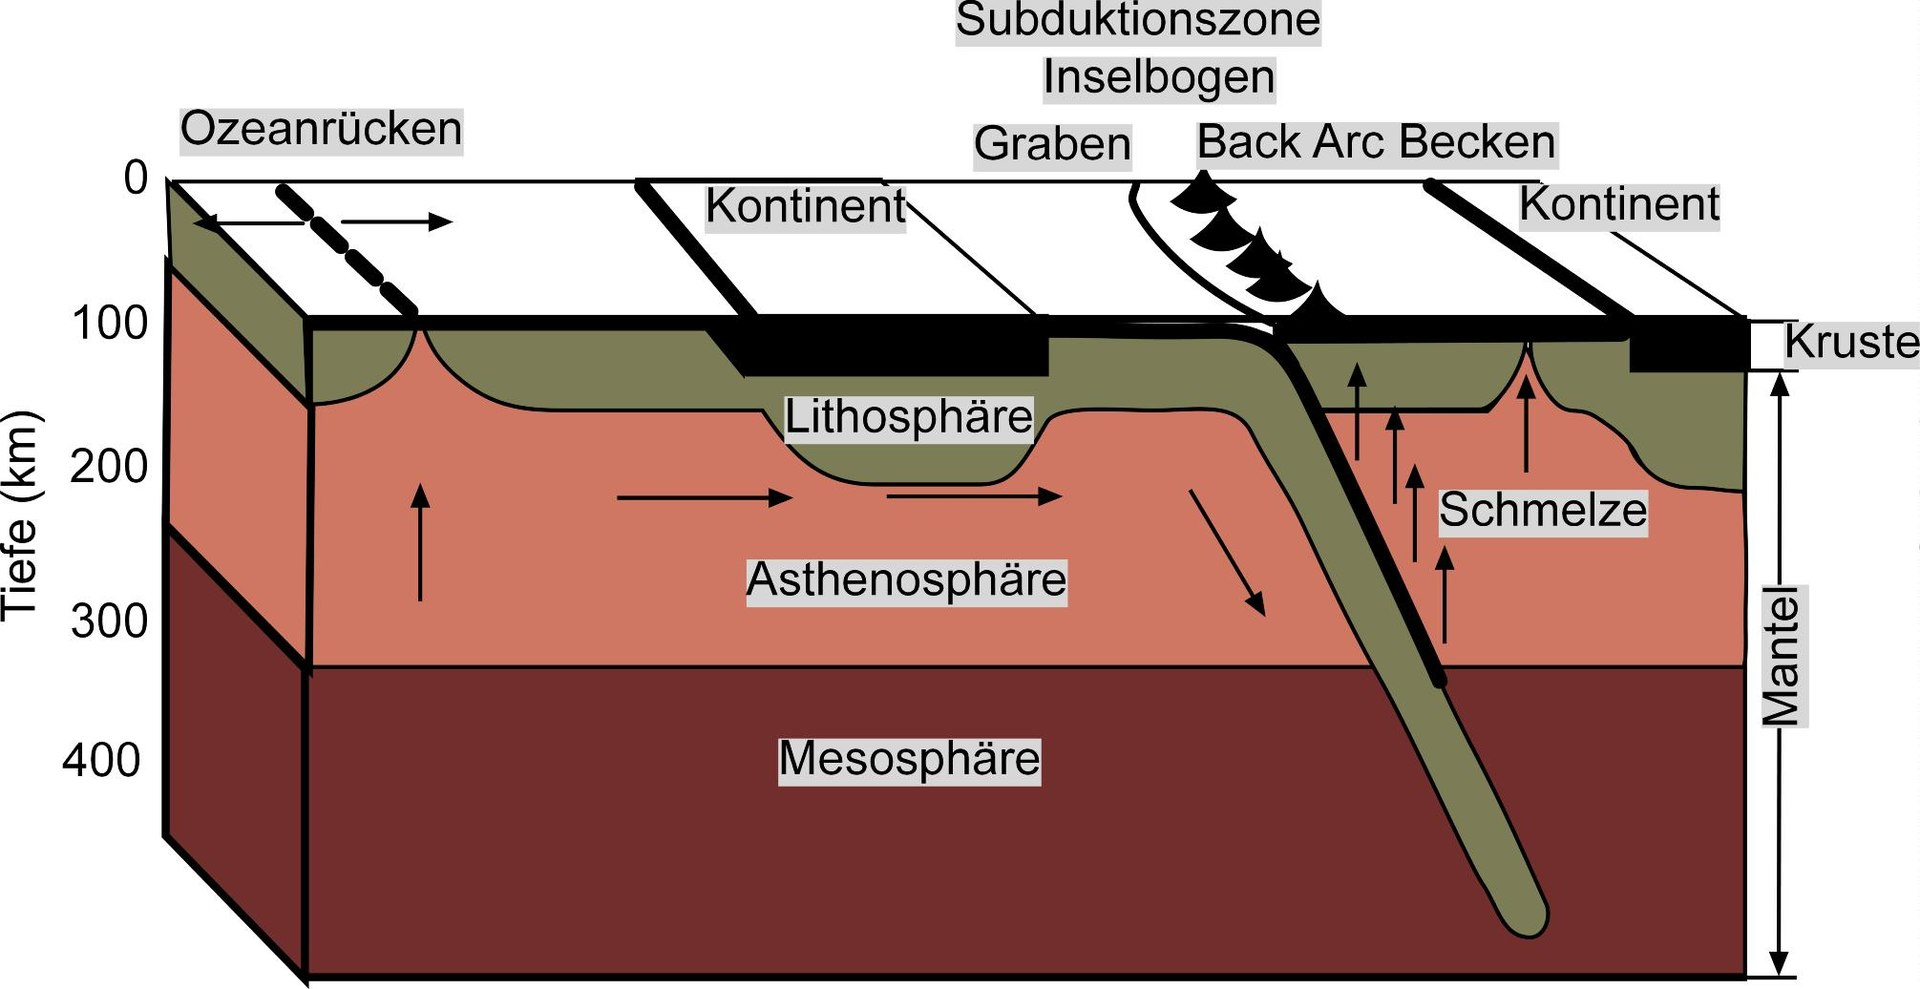
\includegraphics[width=0.9\textwidth]{Plattentekt.jpg}
    \caption{Schematische Darstellung der Dynamik von Lithosphärenplatten: Divergenz an Mittelozeanischen Rücken und Konvergenz an Subduktionszonen - [Gunnar Ries]}
\end{figure}

In einer Analyse von mehr als 35.000 weltweiten Katastrophenereignissen in den Jahren zwischen 1900 und 2015 des Karlsruher Institut für Technologie (KIT) zeigte sich, dass Erdbeben für 26\% der Schäden verantwortlich waren.
Der größte Schaden trat jedoch durch das Tohoku-Erdbeben am 11. März 2011 vor Honshū, Japan auf. Der Schaden durch das Erdbeben und den dadurch ausgelösten Tsunami belief sich auf 18.500 Tote und einen direkten wirtschaftlichen Schaden von etwa 296 Milliarden Euro. 450.000 Menschen wurden obdachlos. \cite{DANIELL}

Aufgrund des Erdbeben kam es zu der Fukushima-Nuklearkatastrophe im Atomkraftwerk Fukushima Daiichi.

Erdbebensicheres Design ist also von wirtschaftlicher und sicherheitstechnischer Bedeutung, um die Aufgabe von Gebäuden zum Schutz des Menschen vor Naturereignissen und ein effektives Tragverhalten zu gewährleisten.

Die Ziele das Eurocode 8 sind daher das Schützen menschlichen Lebens, Schadensbegrenzung und das Aufrechthalten des Betriebs von Strukturen, die zum zivilen Schutz dienen. Beispielsweise sollten Krankenhäuser keine großen Schäden davontragen und den Betrieb nach dem Ereignis fortsetzen können, um ihren Aufgaben im Katastrophenschutz unmittelbar weiter nachzugehen.
Diese Anforderung der Wichtigkeit einer Struktur wird im Bedeutungsbeiwert erfasst. \cite{EC8}

\section{Berechnung}
\label{sec:berechnung}

Grundlegend unterscheidet der Eurocode 8 vier verschiedene Berechnungsmethoden.

\begin{itemize}
  \item Vereinfachtes Antwortspektrenverfahren
  \item Antwortspektrenverfahren unter Berücksichtigung mehrerer Schwingungsformen (Modalanalyse)
  \item Kapazitätsspektrenmethode
  \item Zeitschrittberechnung
\end{itemize}

Da die beiden letzteren Verfahren ein genaueres Gebäudemodell voraussetzen und deutlich aufwändiger sind als die Antwortspektrenverfahren, eignen sich diese nur schwer für die Vordimensionierung von Strukturen. 
Hier werden weiterhin nur die vereinfachten Verfahren mittels Antwortspektren und Modalanalyse betrachtet, die Kapazitätsspektrenmethode und Zeitschrittberechnung sollen aber kurz erläutert werden.

\pagebreak

\subsection{Vereinfachtes Antwortspektrenverfahren}
\label{sec:Antwortspektrenverfahren}

Dieses Verfahren kann nur angewandt werden, wenn die Anforderungen aus dem Eurocode 8 an die Regelmäßigkeit des Grund- und Aufrisses erfüllt sind.
Hier wird nur die Grundschwingung der Struktur berücksichtigt. Daher kann dieses Verfahren nur angewendet werden, wenn die höheren Schwingungsformen keinen wesentlichen Einfluss haben.

Die Grundschwingzeit kann in einer Näherung nach Müller/Keintzel bestimmt werden.

\begin{equation*}
T_1 = \frac{2 \pi H^2}{\alpha_1^2}\sqrt{\frac{m}{hEI}}
\end{equation*}

\thinspace

\begin{multicols}{2}
\makebox[0.8cm]{$H$} Gestamthöhe des Bauwerks \par
\makebox[0.8cm]{$h$} Geschosshöhe \par
\makebox[0.8cm]{$m$} Geschossmasse \par
\makebox[0.8cm]{$EI$} Steifigkeit \par 
\makebox[0.8cm]{$\alpha_1$} Schwingzeitbeiwert \par
\columnbreak
\begin{flushright}
\begin{tabular}{ |c|c| } 
 \hline
 Geschosszahl & $\alpha_1$ \\
 \hline\hline
 1 & 1.32 \\ 
 2 & 1.53 \\ 
 5 & 1.71 \\ 
 10 & 1.78 \\ 
 \hline
\end{tabular}
\end{flushright}
\end{multicols}

Mit der Grundschwingzeit kann nun aus dem Antwortspektrum (\cref{sec:Antwortspektren}) der Bemessungswert der Spektralbeschleunigung $S_d$ bestimmt und die Gesamterdbebenkraft $F_b$ brechnet werden.

\begin{figure}[H]
    \centering
    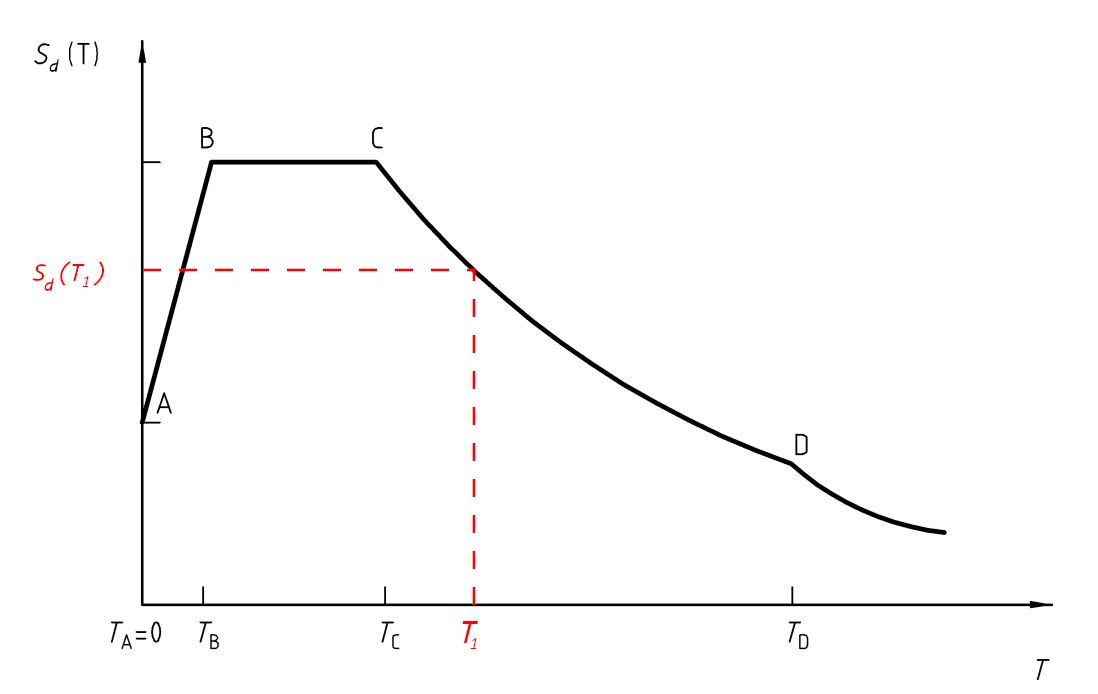
\includegraphics[width=0.9\textwidth]{AWS_Einleitung.png}
    \caption{Bemessungsspektrum}
\end{figure}

\pagebreak

\begin{equation*}
F_b = S_d(T_1) \cdot M \cdot \lambda
\end{equation*}

$M$ ist die Gesamtmasse des Bauwerks und $\lambda$ der Korrekturfaktor von 0.85 für $T_1 \leq 2T_c$ für Gebäude mit mehr als zwei Geschossen und sonst $\lambda=1.0$.
Die Grundschwingungsform darf linear angenähert werden. Somit können die angreifenden Horizontalkräfte vereinfacht linear über die Geschosse verteilt werden.

\begin{minipage}{0.6\textwidth}

\begin{equation*}
F_i = F_b \cdot \frac{z_i m_i}{\sum z_i m_i}
\end{equation*}

\vspace{2ex}
\vspace{2ex}

\makebox[0.8cm]{$F_i$}  Am Geschoss $i$ angreifende Horizontalkraft\par
\makebox[0.8cm]{$z_i$}  Höhen vom Boden zu den Geschossen\par
\makebox[0.8cm]{$m_i$}  Geschossmassen\par

\end{minipage}%
\hfill
\begin{minipage}{0.4\textwidth}

\begin{flushright}
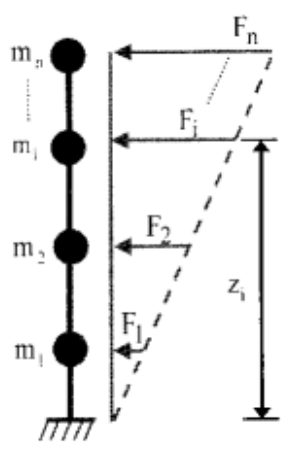
\includegraphics[width=0.4\linewidth]{Fi.png}
\end{flushright}

\end{minipage}%

Mit den Horizontalkräften können nun die Nachweise der Standsicherheit geführt werden.

\subsection{Antwortspektrenverfahren unter Berücksichtigung mehrerer Schwingungsformen (Modalanalyse)}
\label{sec:Modalanalyse}

Sind die Bedingungen an die Regelmäßigkeit des Bauwerks nicht erfüllt und es sollen mehr Schwingungsformen, zum Beispiel auch an einem dreidimensionalen Modell, betrachtet werden, so kann eine Modalanalyse durchgeführt werden.

Das Vorgehen ist ähnlich zu \cref{sec:Antwortspektrenverfahren}, jedoch wird für jede Schwingungsform die Periode ermittelt, eine Spektralbeschleunigung bestimmt und die Horizontallasten anhand der Beteiligungsfaktoren der Schwingungsform angesetzt.

\begin{figure}[H]
    \centering
    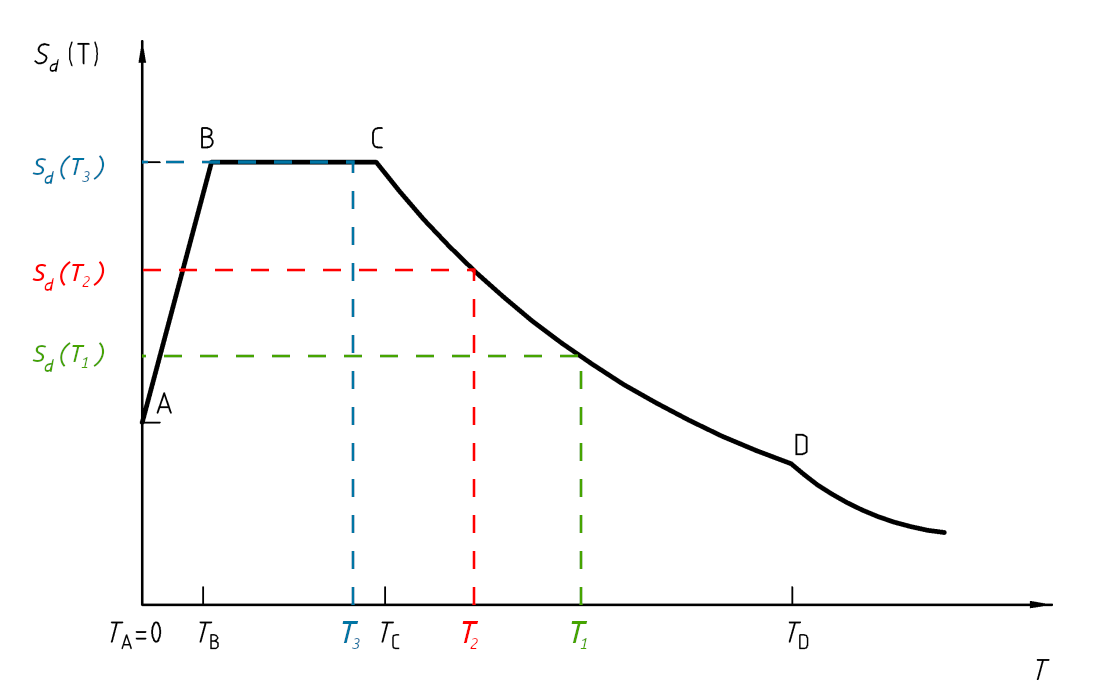
\includegraphics[width=0.9\textwidth]{AWS_Modal_Einleitung.png}
    \caption{Bemessungsspektrum Modalanalyse}
\end{figure}

\begin{figure}[H]
    \centering
    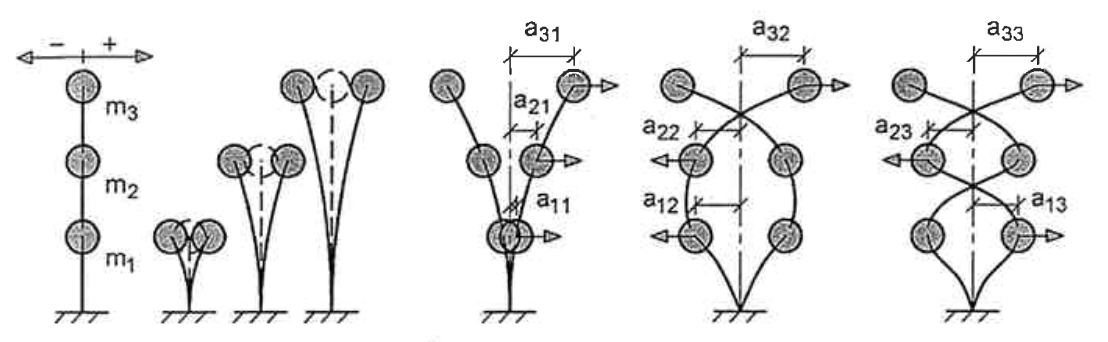
\includegraphics[width=0.9\textwidth]{Beteiligungsfaktoren.png}
    \caption{Eigenschwingungsformen eines Dreimassensystems \cite{Pocanschi}}
\end{figure}

Anschließend müssen die modalen Schnittgrößen und Verschiebungen kombiniert werden. Hier sieht der Eurocode die SRSS-Methode (Square Root of Sum of Squares)

\begin{equation*}
S = \sqrt{\sum_{j=1}^{n}S_j^2}
\end{equation*}

und die CQC-Methode (Complete Quadratic Combination)

\begin{equation*}
S = \sqrt{\sum_{j=1}^{n}\sum_{k=1}^{n} S_j \cdot \rho_{jk} \cdot S_k}
\end{equation*}

vor. Hier ist $\rho_{jk}$ der Wechselwirkungsfaktor, der sich für konstante $\xi_j = \xi_k = \xi$ wie folgt berechnet.

\begin{equation*}
\rho_{jk} = \frac{8 \xi^2 (1 + r) r^{3/2}}{(1 - r^2)^2 + 4 \xi^2 r ( 1 + r)^2}
\quad\mathrm{mit}\quad 
r = \frac{\omega_k}{\omega_j}
\end{equation*}

Neben der CQC-Methode darf auch die CQCi-Methode angewendet werden, welche eine Modifikation unter Berücksichtigung des Vorzeichens der i-ten Eigenform darstellt.

\pagebreak

\subsection{Kapazitätsspektrenmethode}
\label{sec:Kapazitaetsspektrenmethode}

Die auch als \glqq pushover analysis\grqq{} bezeichnete Methode ist ein nicht-elastisches statisches Verfahren unter Berücksichtung des Eigengewichts und monoton ansteigender horizontaler Lasten zur Bestimmung der Grenzlast über die Grenzduktilität.
Sie ist ein genaueres Verfahren zur Bestimmung der plastischen Kapazität, die in den vereinfachten Verfahren von dem Verhaltensbeiwert $q$ erfasst werden.

\subsection{Zeitschrittberechnung}
\label{sec:Zeitschrittberechnung}

Die Berechnung mittels Zeitschrittverfahren (\glqq time-history analysis\grqq{}) ist ein nicht-lineares Verfahren, welches eine zeitabhängige Antwort einer Struktur über die direkte numerische Integration der Differentialgleichungen der Bewegung unter den im Eurocode 8 angegebenen simulierten oder tatsächlich aufgezeichneten Akzelerogrammen der Bodenbeschleunigung bestimmt. 

\pagebreak

\section{Bestimmung des Antwortspektrums}
\label{sec:Antwortspektren}

Zur Gewinnung des Antwortspektrums wird ein Einmassenschwinger unter Fußpunktanregung durch ortsspezifische Akzelerogramme betrachtet und dessen Eigenfrequenz variiert.

\begin{figure}[H]
    \centering
    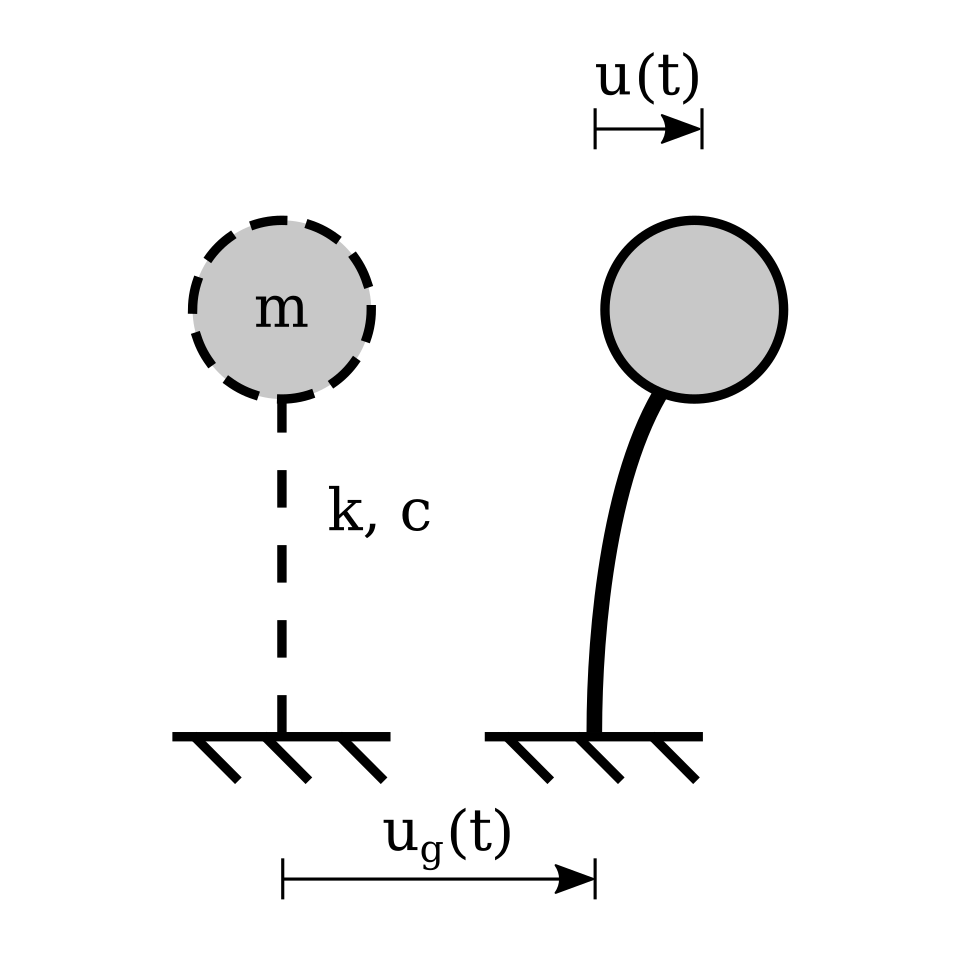
\includegraphics[width=0.4\textwidth]{1MS_AWS.png}
    \caption{Einmassenschwinger mit Fußpunktanregung}
\end{figure}

Die Bewegungsgleichung des Systems

\begin{equation} \label{ems_aws}
m \ddot u + c \dot u + k u = -m \ddot u_g
\end{equation}

nach Umformung mit $\xi = c/(2m\omega)$ und $\omega = \sqrt{k/m}$

\begin{equation} \label{ems_aws_umf}
\ddot u + 2\xi\omega \dot u + \omega^2 u = - \ddot u_g
\end{equation}

zeigt, dass die Antwort lediglich von $\omega$, der Anregung $\ddot u_g$ und $\xi$ abhängig ist, wobei $\xi$ mit 5\% angenommen wird.
Das Antwortspektrum stellt die Einhüllende des Maximalwertes der Absolutbeschleunigung der Systemantwort $S_a=max|\ddot u + \ddot u_g|$ über die Eigenfrequenz des Systems $\omega$ dar. \cite{Bachmann}

Sie wird über die Eckperioden $T_B, T_C, T_D$ und den Bemessungswert der Bodenbeschleunigung $a_g$ parametrisiert. Hinzu kommt noch der Bedeutungsbeiwert $\gamma_1$, der Einfluss des Baugrundes über den Bodenparameter $S$ und ein Dämpfungs-Korrekturbeiwert $\eta$, der bei 5\% viskoser Dämpfung $1.0$ beträgt und sonst mit $\eta=\sqrt{10/(5+\xi)}\geq 0.55$ angegeben wird.

Die Ortsgebundenheit spiegelt sich in den Baugrundverhältnissen und der Bodenbeschleunigung wider. Die Erdbebenzone kann aus einer Karte oder Kartei entnommen werden und liefert den Referenz-Spitzenwert der Bodenbeschleunigung $a_g$.

\begin{table}[H]
\centering
\begin{tabular}{ |c|c| } 
 \hline
 Erdbebenzone & $a_g [m/s^2]$ \\
 \hline\hline
 Zone 0 & - \\ 
 Zone 1 & 0.4 \\ 
 Zone 2 & 0.6 \\ 
 Zone 3 & 0.8 \\ 
 \hline
\end{tabular}
\caption{Tabelle NA.3 — Zuordnung von Referenz-Spitzenwerten der Bodenbeschleunigung zu den Erdbebenzonen [DIN EN 1998-1/NA:2011-01]}
\end{table}

Über die Baugrundverhältnisse kann nach Eurocode 8 NAD eine Baugrundklasse ermittelt werden und in dessen Abhängigkeit Parameter für den Bodenparameter $S$ und die Eckperioden $T_B, T_C, T_D$ angegeben werden.

\begin{table}[H]
\centering
\begin{tabular}{ |c|c|c|c|c| } 
 \hline
 Baugrundklasse & $S$ & $T_B [s]$ & $T_C [s]$ & $T_D [s]$\\
 \hline\hline
 A-R  & 1.00 & 0.05 & 0.20 & 2.0\\ 
 B-R  & 1.25 & 0.05 & 0.25 & 2.0\\ 
 C-R  & 1.50 & 0.05 & 0.30 & 2.0\\ 
 \hline
 B-T  & 1.00 & 0.10 & 0.30 & 2.0\\
 C-T  & 1.25 & 0.10 & 0.40 & 2.0\\
 \hline
 C-S  & 0.75 & 0.10 & 0.50 & 2.0\\
 \hline
\end{tabular}
\caption{Tabelle NA.4 — Werte der Parameter zur Beschreibung des elastischen horizontalen Antwortspektrums [DIN EN 1998-1/NA:2011-01]}
\end{table}

Der Bedeutungsbeiwert bildet die Wichtigkeit einer Struktur ab und erhöht die Wiederkehrperiode bei einer Auftretenswahrscheinlichkeit $P_R$ von 10\% in einer Zeitspanne $T_L$ von 50 Jahren.
Bei einem Bedeutungsbeiwert von $\gamma_1 = 1.0$ beträgt die mittlere Wiederkehrperiode $T_R$

\begin{align*}
T_R &= \frac{-T_L}{ln(1 - P_R)}\\
    &= \frac{-50}{ln(1 - 0.1)}\\
    &=  475 \mbox{ Jahre}
\end{align*}

\begin{table}[H]
\centering
\begin{tabular}{ |c|p{7cm}|c|c| } 
 \hline
 Bedeutungskategorie & Bauwerke & $\gamma_1$ & $T_R$ [a]\\
 \hline\hline
 I   & Bauwerke ohne Bedeutung für den Schutz der Allgemeinheit, mit geringem Personenverkehr (z. B. Scheunen, Kulturgewächshäuser, usw.). & 0.8 & 225\\
 \hline
 II  & Bauwerke, die nicht zu den anderen Kategorien gehören ( z. B. kleinere Wohn- und Bürogebäude, Werkstätten, usw.). & 1.0 & 475\\
 \hline
 III & Bauwerke, von deren Versagen bei Erdbeben eine große Zahl von Personen betroffen ist ( z. B. große Wohnanlagen, Schulen, Versammlungsräume, Kaufhäuser, usw.). & 1.2 & 820\\
 \hline
 IV  & Bauwerke, deren Unversehrtheit im Erdbebenfall von hoher Bedeutung für den Schutz der Allgemeinheit ist ( z. B. Krankenhäuser, wichtige Einrichtungen des Katastrophenschutzes, der Feuerwehr und der Sicherheitskräfte, usw.). & 1.4 & 1300\\
 \hline
\end{tabular}
\caption{Tabelle NA.6 — Bedeutungskategorien und Bedeutungsbeiwerte [DIN EN 1998-1/NA:2011-01]}
\end{table}

Das elastische Antwortspektrum $S_e(T)$ wird somit über folgende Ausdrücke bestimmt.

\begin{align*}
T_A \leq T \leq T_B: S_e(T) &= a_g\gamma_1S \left[ 1+\frac{T}{T_B}(\eta2.5-1) \right] \\
T_B \leq T \leq T_C: S_e(T) &= a_g\gamma_1S\eta2.5\\
T_C \leq T \leq T_D: S_e(T) &= a_g\gamma_1S\eta2.5\frac{T_C}{T}\\
T_D \leq T: S_e(T) &= a_g\gamma_1S\eta2.5\frac{T_CT_D}{T^2}
\end{align*}

\begin{figure}[H]
    \centering
    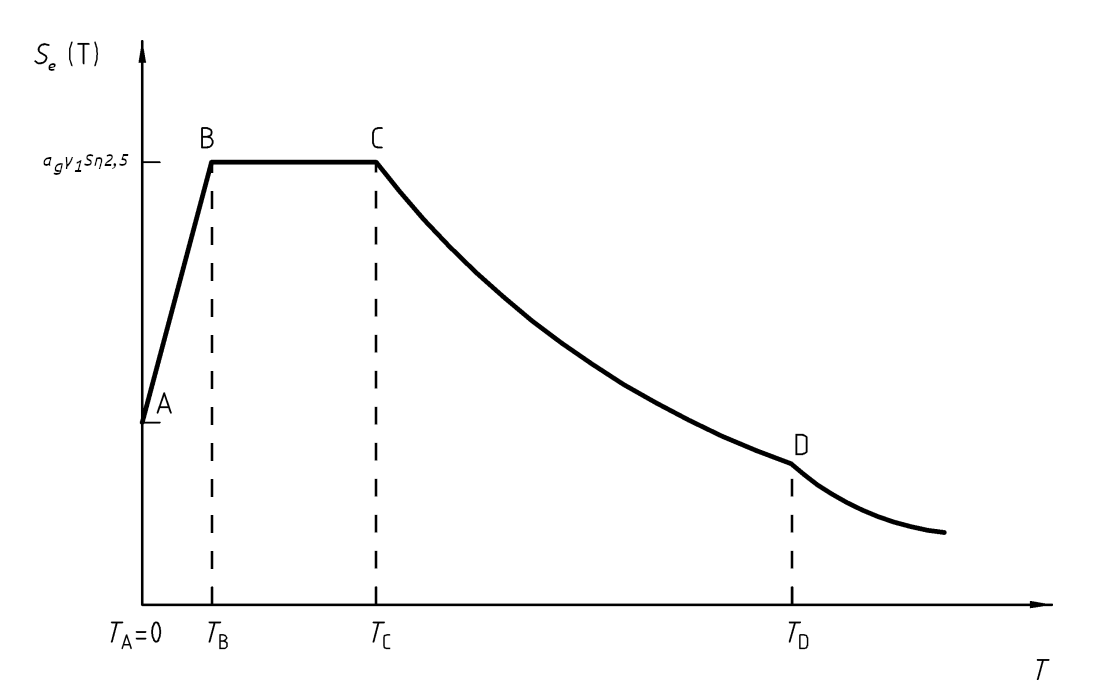
\includegraphics[width=0.9\textwidth]{AWS_Elastisch_Perioden.png}
    \caption{Elastisches Antwortspektrum}
\end{figure}

\pagebreak


\chapter{Dämpfer und Isolatoren}
Wenn die Einwirkungen aus Erdbeben sehr groß sind, zum Beispiel durch eine hohe Anforderung an den Bedeutungsbeiwert oder wenn sich das Bauwerk in einem Starkbebengebiet befindet, ist es meistens technisch und wirtschaftlich günstiger, die Struktur von der Einwirkung zu isolieren, damit sie dieser nicht mehr vollends ausgesetzt wird.

Es können leichtere Konstruktionen gebaut werden, die durch geringere Aufwendung an Material die Kosten senken und die Nachhaltigkeit durch Senken des Ausstoßes an CO\textsubscript{2} erhöhen.

Die horizontale Isolation ist keine Lösung der Neuzeit. Schon die Baumeister im alten China ordneten zwischen Fundament und Grundplatte eine Schicht aus rolligem Sand an. \cite{Taylor}\\
Im 20. Jahrhundert folgten einige Patente mit dem selben Grundprinzip und 1921 realisierte Frank Lloyd Wright das Imperial Hotel in Tokyo mit einer Isolation mittels einer 3m mächtigen Schicht aus Weichboden. Das Gebäude überstand ein zwei Jahre später aufgetretenes schweres Erdbeben nahezu unbeschadet. \cite{Reitherman}

Für die Isolierung stehen einige verschiedene Mechanismen, wie zum Beispiel kinematische Lager, Gleitpendelisolatoren und Elastomerlager (ggf. mit Bleikern zur Erhöhung der Energiedissipation) zur Verfügung.
In dieser Arbeit sollen nur Gleitpendelisolatoren betrachtet werden.

\pagebreak

\section{Gleitpendelisolatoren}
\label{sec:gleitisolatoren}

 Gleitpendelisolatoren bestehen aus zwei spherisch angeformten Lagerplatten, zwischen denen ein Gleitschuh geschaltet wird.

\begin{figure}[H]
    \centering
    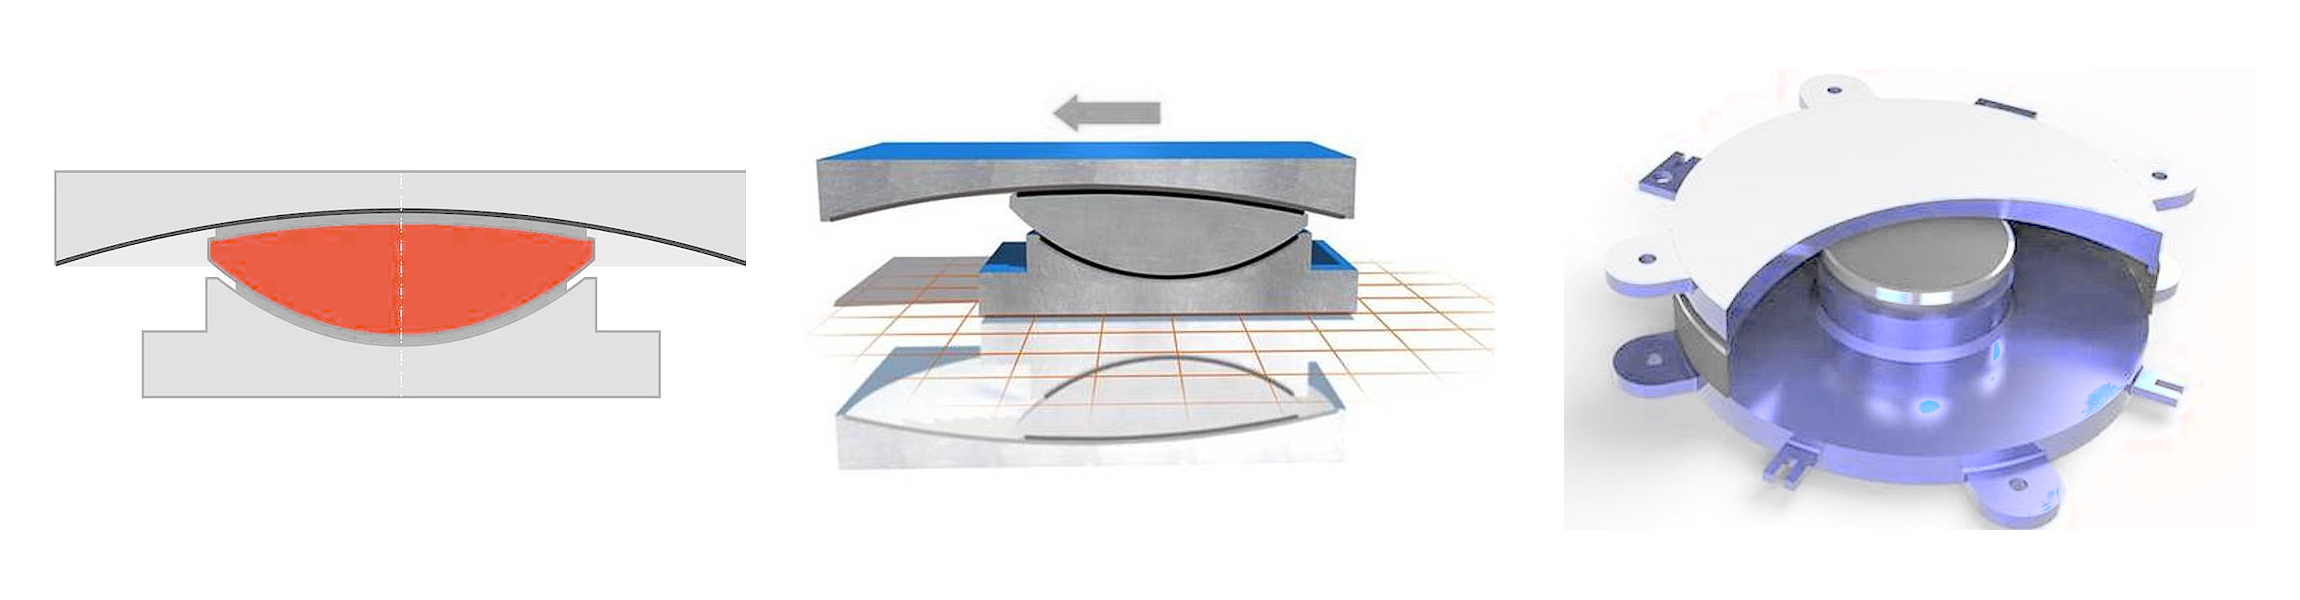
\includegraphics[width=0.9\textwidth]{maurer.png}
    \caption{Gleitpendelisolator [Maurer SE (maurer.eu)]}
\end{figure}

Die Reibung zwischen den Schnittstellen und somit die Energiedissipation kann eingestellt werden.
Bei einem zu hohen Reibkoeffizienten besteht jedoch die Gefahr, dass die Rückzentrierung nicht mehr gewährleistet werden kann, welche ein großer Vorteil der Gleitpendelisolatoren ist.
Zur Erhöhung der Dissipation können aber auch zusätzliche viskose Dämpfungselemente angeordnet werden (\cref{Dampener}).

\begin{figure}[H]
    \centering
    \subfloat[Gleitpendelisolator]{{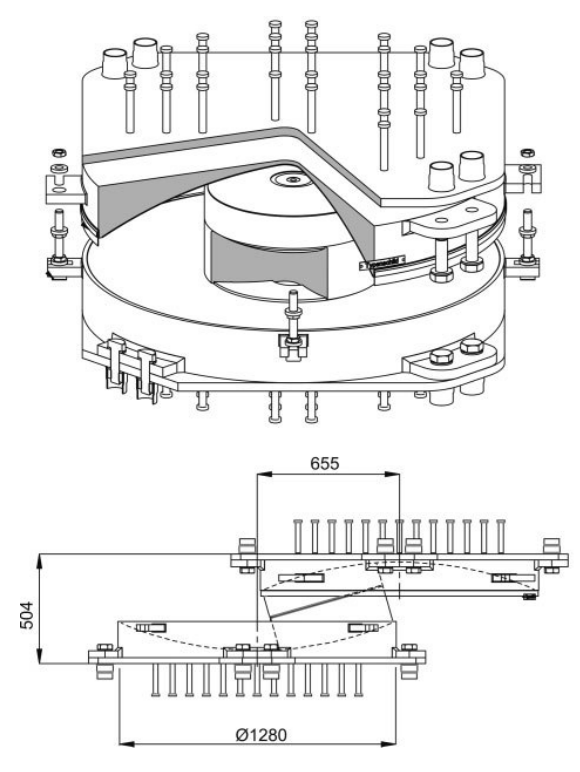
\includegraphics[width=0.45\linewidth]{Algerien_1.png} }}%
    \qquad
    \subfloat[Viskoser Hydraulikdämpfer]{{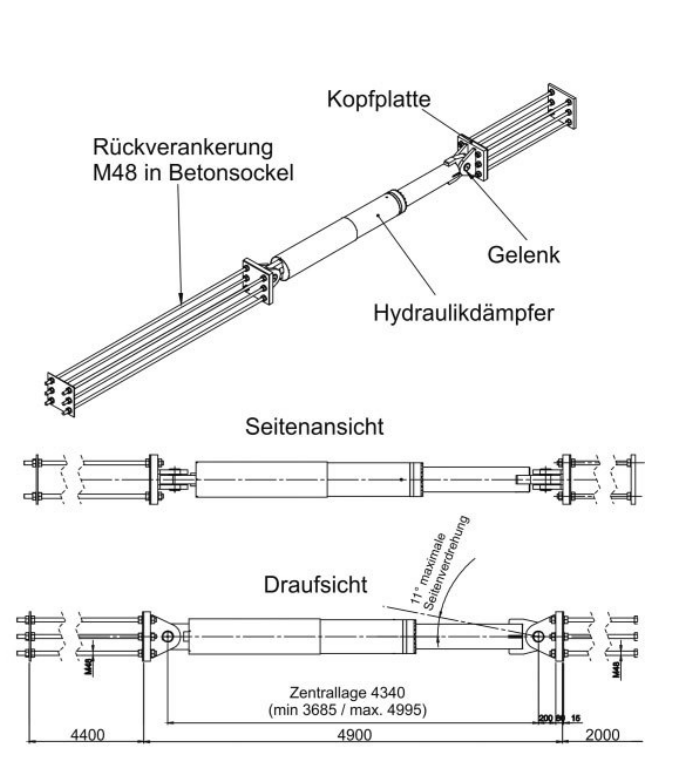
\includegraphics[width=0.45\linewidth]{Algerien_2.png} }}%
    \caption{Bauform der Iolatoren (a) und Dämpfer (b) der Großen Moschee von Algerien \cite{AKK}}%
\end{figure}

\begin{figure}[H]
    \centering
    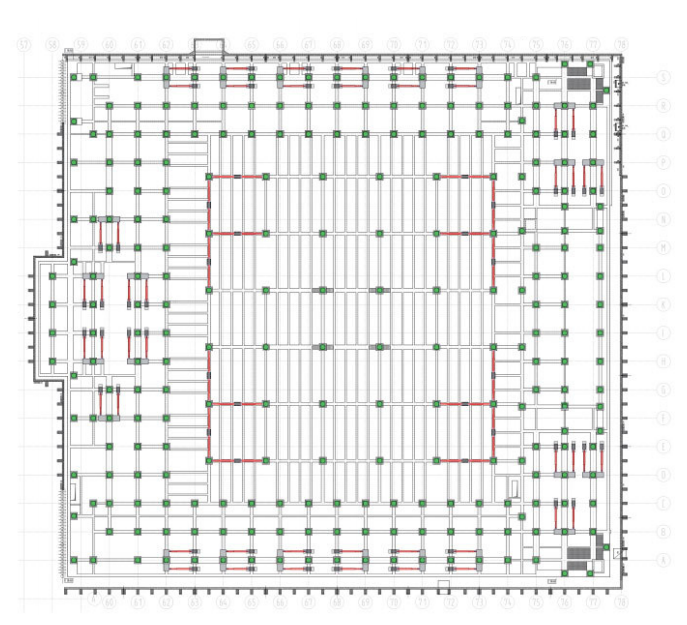
\includegraphics[width=0.9\textwidth]{Algerien_3.png}
    \caption{Verteilung der Isolatoren (grün) und Dämpfer (rot) im Grundriss \cite{AKK}}
	\label{Dampener}
\end{figure}

\pagebreak

\section{Funktionsweise}
\label{sec:funktion}

Isolatoren stellen eine Ebene zwischen der Gründung und dem aufgehendem Bauwerk dar. Sie haben eine deutlich geringere Steifigkeit als die zu isolierende Struktur, wodurch zwar große Verschiebungen am Isolator auftreten (\cref{Verteilung}), aber die Grundschwingzeit reduziert wird.
Die relativen Verschiebungen der Struktur werden verringert und somit die Beschleunigungen und ebenso die Trägheitskräfte der Massen reduziert.

\begin{figure}[h]
    \centering
    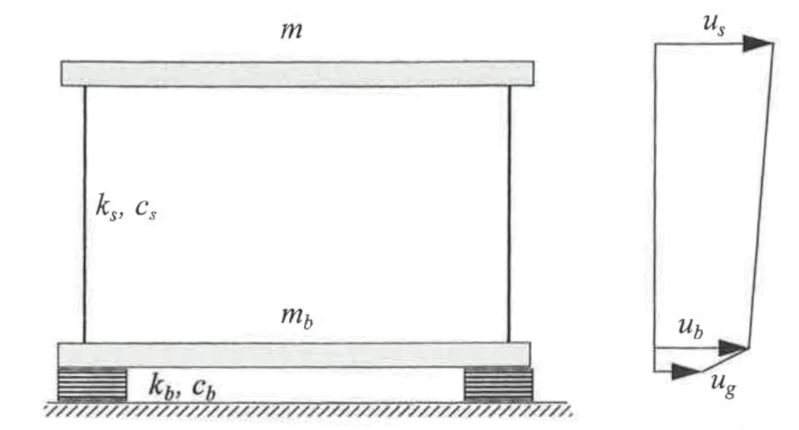
\includegraphics[width=0.9\textwidth]{Verschiebung_iso.png}
    \caption{Verteilung der Verschiebungen an einem isolierten System \cite{Kelly}}
	\label{Verteilung}
\end{figure}

Die Dissipationsfähigkeit, Steifigkeit und Eigenfrequenz dieser Isolatoren können über den Reibkoeffizienten, den Radius des Pendels und die Masse über dem Isolator beeinflusst werden.

\subsection{Abstimmung}
\label{sec:abstimmung}

Damit der Isolator möglichst effektiv wirkt, sollte das Ziel sein, die Masse direkt über dem Isolator möglichst groß zu wählen und die Steifigkeit zu reduzieren, wobei die aufgehende Struktur möglichst steif sein sollte.
Dadurch sollte die Periode des Isolators $T_I$ möglichst weit von der Periode der Struktur $T_S$ entfernt sein.
Ein Wert, der sich in der Praxis als anstrebenswert erwiesen hat, ist $T_I \approx 3 \cdot T_S$.

\pagebreak

\subsection{Steifigkeit}
\label{sec:steifigkeit}

Die effektive Steifigkeit kann über die Rückstell- und Reibkraft des Gleitpendellagers berechnet werden. Die Rückstellkraft wird durch die Anhebung der Vertikalkraft (Eigengewicht des Bauwerks) ausgelöst. \cite{Pocanschi}

\begin{figure}[H]
    \centering
    \includegraphics[width=0.9\textwidth]{Pendellager.png}
    \caption{Schematischer Aufbau des Gleitpendellagers im zentriertem sowie im ausgelenkten Zustand \cite{Romen}}
\end{figure}

\begin{align*}
F_{\text{Rück}} &= \frac{G D}{R \cos \theta}\\
F_{\text{Reib}} &= \mu G
\end{align*}

\makebox[0.8cm]{$G$}  Vertikalkraft (Eigengewicht)\par
\makebox[0.8cm]{$D$}  Auslenkung\par
\makebox[0.8cm]{$R$}  Radius der Isolator-Gleitfläche\par
\makebox[0.8cm]{$\theta$}  Winkel der Auslenkung\par
\makebox[0.8cm]{$\mu$}  Reibkoeffizient des Isolators\par

Für kleine Winkel mit $\cos \theta = 1$ ergibt sich die Steifigkeit zu:

\begin{align}
k_{eff} &= \frac{F_{\text{Rück}} + F_{\text{Reib}}}{D}\nonumber\\
        &= \frac{G}{R} + \mu \frac{G}{D}\label{keff}
\end{align}

\pagebreak

\subsection{Dämpfung}
\label{sec:daempdung}

Die effektive Dämpfung ergibt sich aus der Fläche der Hystereseschleife und der effektiven Steifigkeit des Gleitpendellagers. \cite{Huber}\cite{Pocanschi}

\begin{figure}[h]
    \centering
    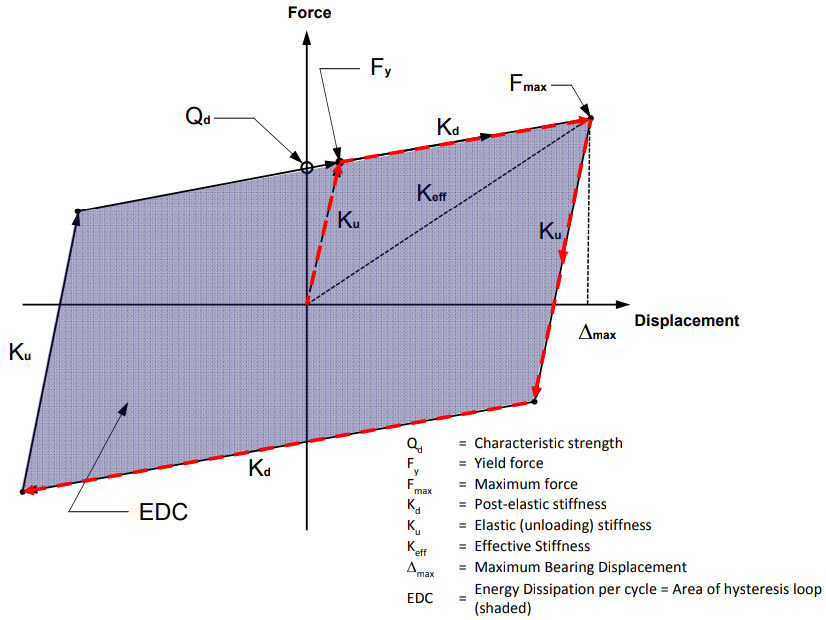
\includegraphics[width=0.9\textwidth]{Hysteresis.png}
    \caption{Hysterese-Zyklus [HDR Engineering Inc.]}
\end{figure}

\begin{align}
\xi_{eff} &= \frac{4 \mu G D}{2 \pi k_{eff} D^2}\nonumber\\
          &= \frac{2}{\pi} \frac{\mu R}{(D + \mu R)}\label{xieff}
\end{align}

Dieser Ansatz hat den Vorteil einer linearen Steifigkeits- und Dämpfungsfunktion, was die spätere Lösung der Differentialgleichungen vereinfacht. In \cref{cap:analyse} werden die Implikationen davon betrachtet.

\pagebreak

\section{Schwierigkeiten bei der Vordimensionierung}
\label{sec:schwierigkeitenvordimensionierung}

Für eine genaue Berechnung ist es sinnvoll, ein Gebäudemodell samt Isolator zu erstellen und mit dem Zeitschrittverfahren und Erdbebenzeitverläufen zu berechnen. Dies ist jedoch sehr aufwendig und bei einer Vordimensionierung nicht immer praktikabel, da sich Parameter noch ändern können oder nicht bekannt sind.
Ein Ansatz ist es, die Gesamtstruktur auf einen Einmassenschwinger mit der effektiven Masse aus Struktur ($m_S$) und Isolator ($m_I$) zu vereinfachen. Er beruht auf der Annahme, dass die Steifigkeit der Struktur sehr hoch ist und die des Isolators $k_I$ die Eigenform somit dominiert. \cite{Kelly2}
Die Eigenfrequenz kann dann mit

\begin{equation}
\omega = \sqrt{\frac{k_I}{m_S + m_I}}
\end{equation}

bestimmt und die Spektralbeschleunigung $Sa(\frac{2 \pi}{\omega})$ aus dem Antwortspektrum entnommen werden.

Soll allerdings eine Modalanalyse am Gebäude mittels EDV vorgenommen werden, wird ein isoliertes Antwortspektrum benötigt.
So könnte man ein grobes Gebäudemodell erstellen und mit dem isolierten Antwortspektrum eine computergestützte Modalanalyse durchführen.

\pagebreak

\chapter{Berechnung des modifizierten Antwortspektrums}
Hier soll nun ein Verfahren hergeleitet und anschließend mit zwei vereinfachten Verfahren verglichen werden. 

Für die Erzeugung der Isolationsspektren wird hier das System um den Isolator erweitert und als Zweimassenschwinger (\cref{fig:vkm}) betrachtet, wobei der obere Schwinger die aufgehende Struktur (1) und der untere Schwinger den Isolator (2) samt des steifen Kellergeschosses beschreiben soll.

\begin{figure}[ht]
    \centering
    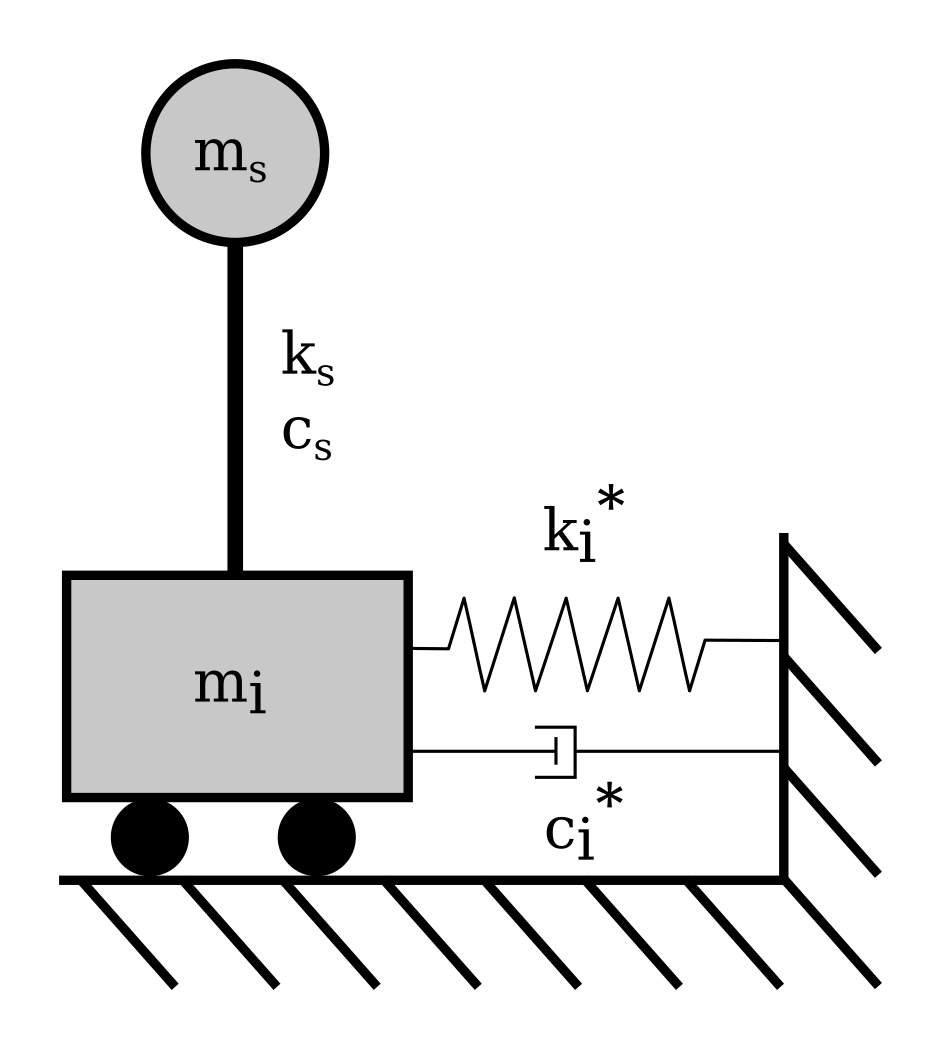
\includegraphics[width=0.5\textwidth]{voigt-kelvin-model.png}
    \caption{Voigt-Kelvin-Modell}
    \label{fig:vkm}
\end{figure}

\section{Ansatz über die Übertragsfunktion}
\label{sec:ansatzfunktion}

Im ersten Ansatz wurde die Möglichkeit untersucht, das Modell in zwei getrennte Systeme zu zerlegen und getrennt zu betrachten.
Die Annahme war, dass der Isolator lediglich als Filter auf das Antwortspektrum wirkt.

\begin{figure}[H]
    \centering
    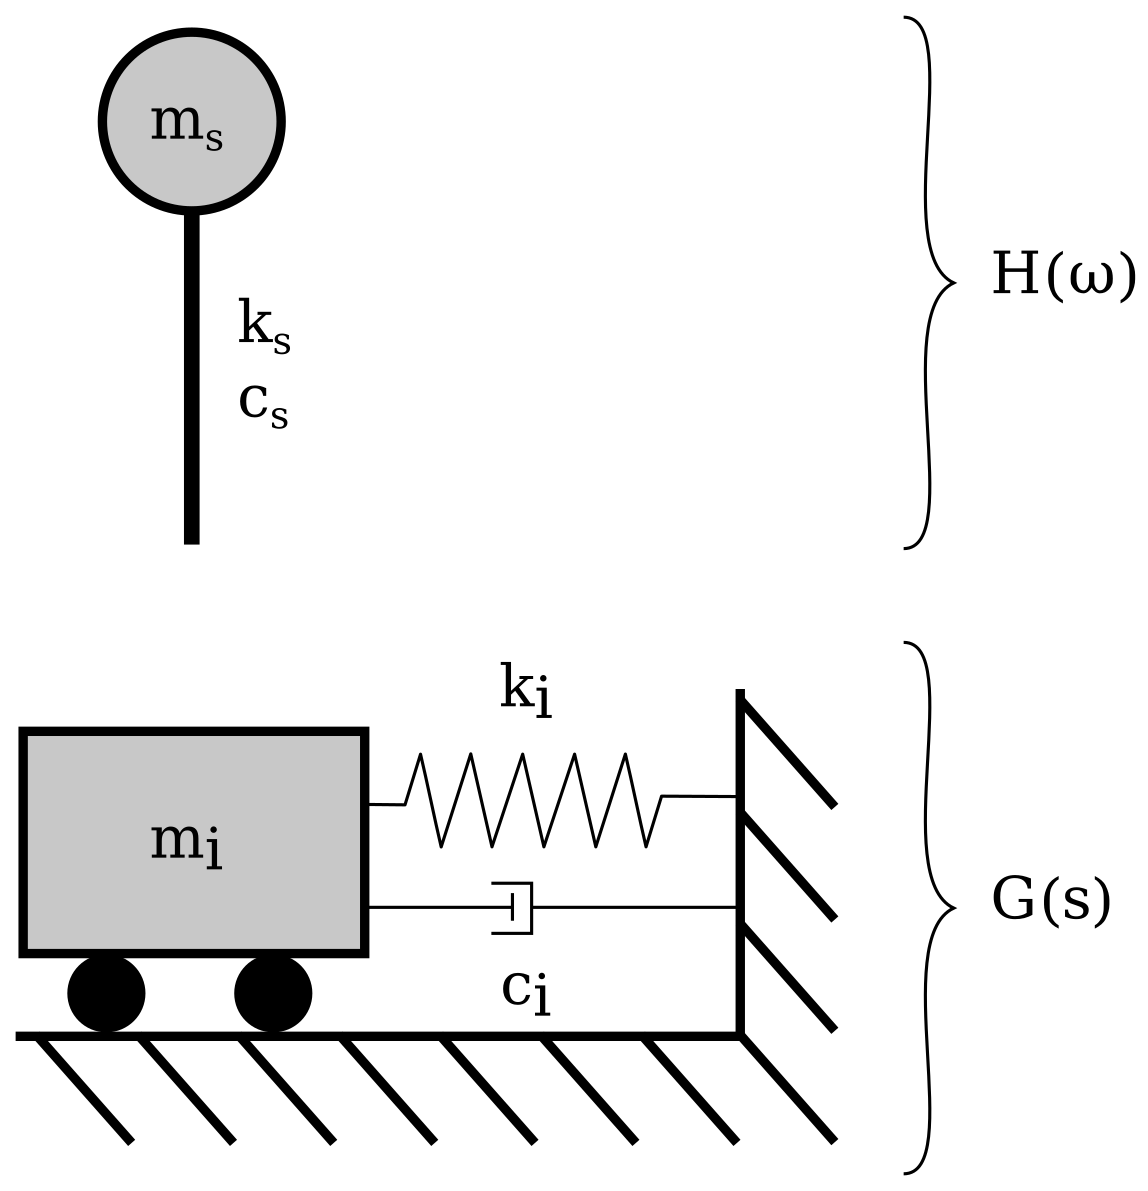
\includegraphics[width=0.7\textwidth]{composition.png}
    \caption{Komposition}
    \label{fig:composition}
\end{figure}

Die Funktion $H(\omega)$ stellt hier das Antwortspektrum dar und $G(s)$ die Übertragungsfunktion des Isolators.
Sie kann mittels der Laplace-Transformation

\begin{equation} \label{laplace}
F(s) = \int_{0}^{\infty} f(t)e^{-st}dt
\end{equation}

aus der Bewegungsgleichung des Isolators \cite{Kramer}

\begin{equation}\label{eq:bewegungsgleichung}
c_i \cdot \dot x(t) + k_i \cdot x(t) = - m_i \cdot \ddot x(t)
\end{equation}

für eine Kraftanregung zu

\begin{equation} \label{laplace2}
G(s)=\frac{X(s)}{F(s)} = \frac{1}{m_i \cdot s^2 + c_i \cdot s + k_i}
\end{equation}

bestimmt (wobei $s = i \omega$) und das isolierte Antwortspektrum ($H(\omega) \cdot |G(s)|$) gewonnen werden, da der Betrag der Übertragungsfunktion den Amplitudengang angibt.

Allerdings war dieser Ansatz nicht zielführend, da (wie an den Bewegungsdifferentialgleichungen (\cref{eq:BewegDGL1} und \cref{eq:BewegDGL2}) erkennbar ist) die Systeme gekoppelt sind und nicht getrennt betrachtet werden können.

\section{Vereinfachter Ansatz}
\label{sec:ansatzvereinfacht}

Zur Ermittelung der Eigenkreisfrequenzen des Zweimassenschwingers $\omega_{L,1,2}$ werden die Verhältniswerte

\begin{align}
\alpha &= \frac{k_2}{k_1} & \beta  &= \frac{m_2}{m_1} \\
\end{align}

eingeführt. Damit lassen sich die Eigenkreisfrequenzen und Perioden des isolierten Systems bezogen auf die Eigenkreisfrequenz $\omega$ des nicht isolierten Bauwerks wie folgt berechnen \cite{Pocanschi} \cite{Isemann}

\begin{align}
\omega_{L,1}^2 &= \frac{1 + \alpha + \beta - \sqrt{(1 + \alpha + \beta)^2 - 4 \alpha \beta}}{2 \beta} \omega^2\\
\omega_{L,2}^2 &= \frac{1 + \alpha + \beta + \sqrt{(1 + \alpha + \beta)^2 - 4 \alpha \beta}}{2 \beta} \omega^2
\end{align}

\begin{align}
T_{L,1} &= \frac{2 \pi}{\omega_{L,1}} & T_{L,2} &= \frac{2 \pi}{\omega_{L,2}}
\end{align}

Die Komponenten der Eigenvektoren $\vec{\Phi}_{1,2}$ lassen sich über die Beiwerte $\alpha$ und $\beta$ bestimmen.

\begin{align}
r_1 &= \frac{1 + \alpha - \beta + \sqrt{(1 + \alpha + \beta)^2 - 4 \alpha \beta}}{2}\\
r_2 &= \frac{1 + \alpha - \beta - \sqrt{(1 + \alpha + \beta)^2 - 4 \alpha \beta}}{2}
\end{align}

Die Schwingungsformen lauten damit wie folgt und können normiert werden.

\begin{align}
\vec{\Phi}_1 &= \binom{1}{r_1} & \vec{\Phi}_2 &= \binom{1}{r_2}\\
\vec{\Phi}_1 &= \binom{1/r_1}{1} & \vec{\Phi}_2 &= \binom{1/r_1}{1}
\end{align}

Der Beteiligunsfaktor der ersten Schwinungsform wird wie folgt definiert.

\begin{equation}
L_1 = \frac{\vec{\Phi}_1^T M \vec{I}}{\vec{\Phi}_1^T M \vec{\Phi}_1}
\end{equation}

Da die Steifigkeit des Isolators idealerweise deutlich geringer als die der Struktur ist gilt $\alpha \rightarrow 0$, $\vec{I} = \binom{1}{1}$ und $L_2$ wird klein, da die Schwingungsform durch die erste bestimmt wird.
Damit lässt sich die maximale absolute Beschleunigung der Massen der ersten Schwingungsform des Zweimassenschwingers infolge einer Fußpunktanregung bestimmen.

\begin{equation}
\ddot U_{max} = \vec{\Phi}_1 L_1 S_a(T_{L,1}, \xi_{L,1})
\end{equation}

Für die Erzeugung des isolierten Antwortspektrums wird die Steifigkeit der Struktur variiert und die Eigenkreisfrequenz dieser ermittelt.

\begin{equation}
k_{1,i} = \frac{4 \pi^2 m_1}{T_i^2}
\end{equation}

\begin{equation}
\omega = \sqrt{\frac{k_1}{m_1}}
\end{equation}

Da die Antwortspektren im Eurocode auf eine Dämpfung von 5\% normiert sind, wird unter der Annahme, dass die Dämpfung des Isolators dominiert, das Antwortspektrum abgemindert.

\begin{equation}\label{eta}
\eta = \sqrt{\frac{10}{5 + \xi_2}}
\end{equation}

\section{Ansatz über die Transmissibilität}
\label{sec:ansatztrasnm}

Die Beschleunigung aus dem Antwortspektrum wird in eine äquivalente harmonische Beschleunigungsanregung am Fußpunkt umgerechnet.
Anschließend wird über die Bewegungsgleichungen (\cref{eq:2DOF1,eq:2DOF2}) das Verhältnis der Amplituden von Fußpunktanregung zu harmonischer Schwingung an der oberen Masse $m_1$ hergeleitet.
Da die Perioden im Antwortspektrum die Eigenfrequenz des zur Erzeugung verwendeten Einmassenschwingers darstellen, kann eine harmonische Anregung erzeugt werden, deren Erregerfrequenz der Eigenfrequenz des Einmassenschwingers entspricht.
Zur Erzeugung eines isolierten Antwortspektrums soll dann die Steifigkeit $k_1$ variiert werden, sodass die Eigenfrequenz des oberen Systems der Periode des Antwortspektrums entspricht, und die Parameter des Isolators konstant bleiben.
So kann ein Isolationsspektrum erzeugt werden, das für jede Periode der aufgehenden Struktur eine äquivalente Beschleunigungsantwort angibt.

\subsection{Transmissibilität}
\label{sec:transm}

Die Bewegungsdifferentialgleichungen für das in \cref{fig:vkm} dargestellte System lauten:

\begin{align}
\ddot x_1 m_1 &= -(x_1 - x_2) k_1 -(\dot x_1 - \dot x_2) c_1 \label{eq:BewegDGL1}\\
\ddot x_2 m_2 &= (x_1 - x_2) k_1 + (\dot x_1 - \dot x_2) c_1 - (x_2 - x_3) k_2 - (\dot x_2 - \dot x_3) c_2 \label{eq:BewegDGL2}
\end{align}

Ansatz für harmonische Schwingung:

\begin{align*}
x_j &= S_j e^{i \omega t} & \dot x_j &= i \omega S_j e^{i \omega t} & \ddot x_j &= - \omega^2 S_j e^{i \omega t}
\end{align*}

\begin{align}
- \omega^2 S_1 m_1 e^{i \omega t} &= - (S_1 - S_2) e^{i \omega t} k_1 - (S_1 - S_2) i \omega c_1 e^{i \omega t} \label{eq:2DOF1} \\
- \omega^2 S_2 m_2 e^{i \omega t} &= (S_1 - S_2)(k_1 + i \omega c_1) e^{i \omega t} - (S_2 - S_3)(k_2 + i \omega c_2) e^{i \omega t} \label{eq:2DOF2}
\end{align}

\cref{eq:2DOF1} nach $S_2$ umgestellt:

\begin{align*}
\omega^2 S_1 m_1 &= (S_1 - S_2)(k_1 + i \omega c_1) \\
&\Rightarrow X_1 = \frac{\omega^2 m_1}{k_1 + i \omega c_1}\\
S_2 &= S_1 (1 - X_1)
\intertext{$S_2$ in \cref{eq:2DOF2} eingesetzt:}
\omega^2 m_2 S_1 &= - (S_1 - S_1 (1 - X_1)) (k_1 + i \omega c_1) + (S_1 (1 - X_1) - S_3) (k_2 + i \omega c_2)\\
&\Rightarrow X_2 = \frac{\omega^2 m_2}{k_2 + i \omega c_2}\\
S_1 (1 - X_1) X_2 &= S_1 (1-X_1) - S_3 - S_1 X_1 \frac{k_1 + i \omega c_1}{k_2 + i \omega c_2}\\
&\Rightarrow X_{12} = \frac{\omega^2 m_1}{k_2 + i \omega c_2}\\
S_1 (1 - X_1)(X_2 - 1) &= S_3 + S_1 X_{12}\\
S_3 &= S_1 [(1 - X_1)(1 - X_2) - X_{12}]
\end{align*}

Mit den komplexwertigen Transmissionskoeffizienten $X_1$, $X_2$ und $X_{12}$ ergibt sich die Transmissibilität aus dem Betrag des Verhältnisses von $S_1$ zu $S_3$.

\begin{equation}\label{eq:VT2DOF}
VT = \left\lvert \frac{S_1}{S_3} \right\rvert = \left\lvert \frac{1}{[(1 - X_1)(1 - X_2) - X_{12}]} \right\rvert
\end{equation}

Ein Hindernis stellen jedoch noch die Dämpfungsbeiwerte $c_1$ und $c_2$ dar.
Ein Ansatz, der hier untersucht werden soll, ist die steifigkeits- und massenproportionale modale Dämpfung. Sie wird auch als Rayleigh-Dämpfung bezeichnet. \cite{Pocanschi}

\subsection{Rayleigh-Dämpfung}
\label{sec:rayleigh}

Bei diesem Ansatz soll eine Proportionalität zwischen der Dämpfungsmatrix $C$ und den generalisierten Massen- und Steifigkeitsmatrizen $M^*$ und $K^*$ verwendet werden.

\begin{equation*}
C^* = \alpha M^* + \beta K^*
\end{equation*}

Wobei $\alpha$ und $\beta$ die Beiwerte der Rayleigh-Dämpfung sind.
$\alpha M$ kann als äußere und der Term $\beta K$ als innere Dämpfung verstanden werden.

Die Bestimmungsgleichungen der Beweirte lauten wie folgt. \cite{Shambhu}

\begin{align*}
\alpha &= \frac{2 \omega_1^* \omega_2^* (\xi_2 \omega_2^* - \xi_1 \omega_1^*)}{\omega_2^{*2} - \omega_1^{*2}}\\
\beta  &= \frac{2 (\xi_1 \omega_2^* - \xi_2 \omega_1^*)}{\omega_2^{*2} - \omega_1^{*2}}
\end{align*}

Um die Eigenkreisfrequenzen $\omega_1^*$ und $\omega_2^*$ zu erhalten, werden zunächst die Eigenkreisfrequenzen am ungedämpften System berechnet und die Eigenvektoren der zugehörigen Eigenformen bestimmt.

Eigenkreisfrequenz des ungedämpften Systems:

\begin{equation*}
\omega_{1,2}^2 = \frac{(k_2 + k_1) m_1 + k_1 m_2 \pm \sqrt{((k_2 + k_1) m_1 + k_1 m_2)^2 - 4 m_2 m_1 k_2 k_1}}{2 m_2 m_1}
\end{equation*}

Eigenvektoren des ungedämpften Systems:

\begin{align*}
\vec{\Phi}_1 &= \binom{\varphi_{11}}{\varphi_{21}} = \binom{1}{\varepsilon_1} & \vec{\Phi}_2 &= \binom{\varphi_{12}}{\varphi_{22}} = \binom{1}{\varepsilon_2}\\
\intertext{mit}
\varepsilon_1 &= \frac{k_2 + k_1 - m_2 \omega_1^2}{k_1} & \varepsilon_2 &= \frac{k_2 + k_1 - m_2 \omega_2^2}{k_1}
\end{align*}

Nach Betragsgröße normierte Eigenvektoren des ungedämpften Systems:

\begin{align*}
\varphi_{11} &= \sqrt{\frac{1}{1 + \varepsilon_1^2}}  &  \varphi_{12} &= \sqrt{\frac{1}{1 + \varepsilon_2^2}}\\
\varphi_{21} &= \varepsilon_1 \varphi_{11}            &  \varphi_{22} &= \varepsilon_2 \varphi_{12}
\end{align*}

Mit Hilfe der Eigenvektoren können die generalisierten Massen und Steifigkeiten ermittelt werden und damit die Eigenkreisfrequenzen.

Generalisierte Massen:

\begin{align*}
m_2^* &= \vec{\Phi}_1^T M \vec{\Phi}_1               &   m_1^* &= \vec{\Phi}_2^T M \vec{\Phi}_2\\
      &= \varphi_{11}^2 m_2 + \varphi_{21}^2 m_1     &         &= \varphi_{12}^2 m_2 + \varphi_{22}^2 m_1
\end{align*}

Generalisierte Steifigkeiten:

\begin{align*}
k_2^* &= \vec{\Phi}_1^T K \vec{\Phi}_1                                                          &   k_1^* &= \vec{\Phi}_2^T K \vec{\Phi}_2\\
      &= \varphi_{11}^2 (k_2 + k_1) - 2 \varphi_{21} \varphi_{11} k_1 + \varphi_{21}^2 k_1      &         &= \varphi_{12}^2 (k_2 + k_1) - 2 \varphi_{22} \varphi_{12} k_1 + \varphi_{22}^2 k_1
\end{align*}

Eigenkreisfrequenzen der zwei Einmassenschwinger:

\begin{align*}
\omega_1^* &= \sqrt{\frac{k_2^*}{m_2^*}}  &  \omega_2^* &= \sqrt{\frac{k_1^*}{m_1^*}}
\end{align*}

Damit ergeben sich die Dämpfungsbeiwerte der Rayleigh-Dämpfung

\begin{align*}
c_1^* &= \alpha m_1^* + \beta k_1^*\\
c_2^* &= \alpha m_2^* + \beta k_2^*
\end{align*}

und die gedämpfte Eigenfrequenz der ersten, durch den Isolator gesteuerten, Eigenform  

\begin{align*}
\omega_{1d} &= \omega_1 \sqrt{1 - \xi_2^2}\\
T_1         &= \frac{2 \pi}{\omega_{1d}} 
\end{align*}

Das System wird nun aus der Modal- zurück in die Normalform transformiert um die Dämpfungsmatrix $C$ zu erhalten. \cite{Rayleigh}

\begin{equation*}
C = \vec{\Phi}^{-T} C^* \vec{\Phi}^{-1}
\end{equation*}

Die Transmissibilität kann damit bestimmt werden.

\begin{equation}
VT(m_2, k_2, c_2, m_1, k_1, c_1)
\end{equation}

\subsection{Erzeugung des isolierten Antwortspektrums}
\label{sec:transmAWS}

Das isolierte Antwortspektrum kann aus dem elastischen Antwortspektrum erlangt werden.
Für jede Periode $T_i$ wird die Steifigkeit der aufgehenden Struktur berechnet, wobei die restlichen Parameter konstant bleiben.

\begin{equation}
k_{1,i} = m_1 (\frac{2 \pi}{T_i})^2
\end{equation}
  
Damit können die Transmissibilität $VT$, die gedämpfte erste Eigenkreisfrequenz $\omega_{1d}$

\begin{align}
\omega_{1d} &= \omega_1 \sqrt{1 - \xi_2^2} \\
T_1 &= \frac{2 \pi}{\omega_{1d}}
\end{align}

und die zugehörige äquivalente Amplitude der Beschleunigung der Fußpunktanregung

\begin{equation}
S_{a,x_3} = Sa(T_1)
\end{equation}

ermittelt werden. Die Ordinate des isolierten Antwortspektrums beträgt dann

\begin{equation}
S_{a,isoliert} = S_{a,x_3} \cdot VT
\end{equation}
  
\pagebreak


\chapter{Beispielberechnung}
Die Ansätze sollen anhand eines konkreten Beispiels verglichen werden. Hierzu werden die Werte aus \cite{Isemann} Kapitel 11.2.3 verwendet.
Die Parameter des Systems lauten:

\makebox[1cm]{$D$}    = 0.35 m \par
\makebox[1cm]{$\mu$}  = 0.04\par
\makebox[1cm]{$m_1$}  = 2486.7 t\par
\makebox[1cm]{$m_2$}  = 1619.5 t\par
\makebox[1cm]{$R$}    = 2.5 m\par

Es soll ein Antwortspektrum mit folgenden Eckperioden und Bodenbeschleunigung verwendet werden.

\makebox[1cm]{$T_B$}  = 0.4 s\par
\makebox[1cm]{$T_C$}  = 1.6 s\par
\makebox[1cm]{$T_D$}  = 2.0 s\par
\makebox[1cm]{$a_g$}  = 3.924 m/s\textsuperscript{2}\par

\begin{figure}[h]
    \centering
    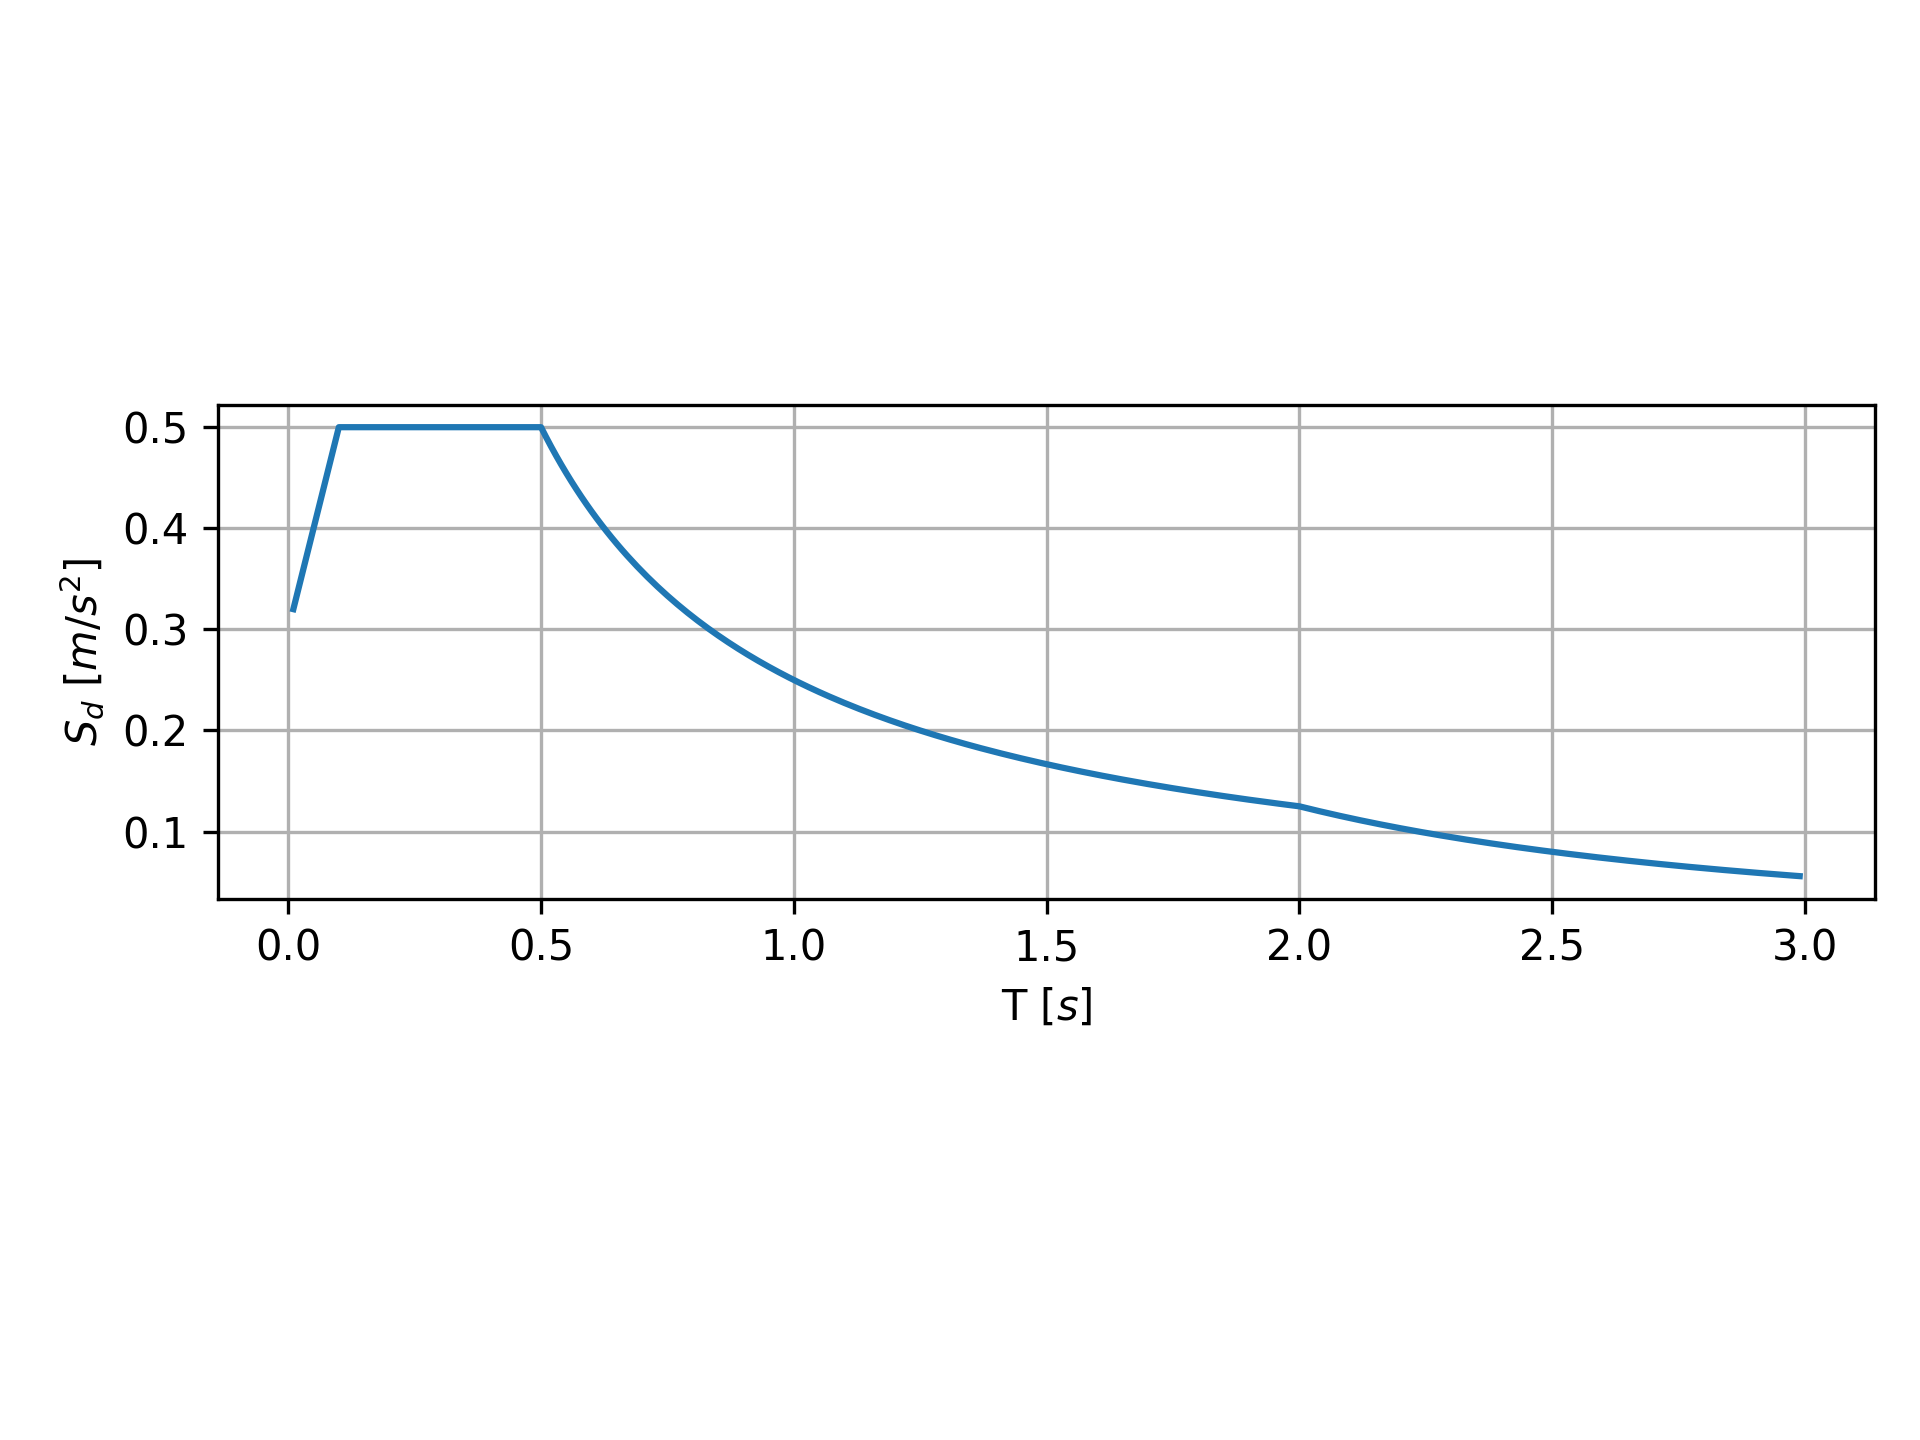
\includegraphics[width=0.9\textwidth]{AWS_beispiel.png}
    \caption{Antwortspektrum (Beispiel 1)}
\end{figure}

Die Steifigkeit $k_2$ ergibt sich aus der effektiven Steifigkeit des Isolators nach \cref{keff}

\begin{equation*}
k_2 = k_{eff} = \frac{G}{R} + \mu \frac{G}{D} = \frac{41062 kN}{2.5 m} + 0.04 \cdot \frac{41062 kN}{0.35 m} = 21117 kN/m
\end{equation*}

Die Dämpfung $\xi_1$ wird mit 5 \% angenommen und die effektive Dämpfung des Isolators $\xi_2$ nach \cref{xieff} bestimmt.

\begin{equation*}
\xi_2 = \xi_{eff} = \frac{2}{\pi} \frac{\mu R}{(D + \mu R)} = \frac{2}{\pi} \frac{0.04 \cdot 2.5 m}{(0.35 m + 0.04 \cdot 2.5 m)} \approx 0.14147
\end{equation*}

\pagebreak

Hier sollen zunächst die Ergebnisse für eine Periode der aufgehenden Struktur von $T = 1 s$ betrachtet werden. Daraus ergibt sich eine Steifigkeit $k_1$ von

\begin{equation*}
k_1 = m_1 (\frac{2 \pi}{T})^2 = 2486.7 t \cdot (\frac{2 \pi}{1 s})^2 = 98170 kN/m
\end{equation*}

\pagebreak

\section{Betrachtung als effektiver Einmassenschwinger}

Wie in \cref{sec:schwierigkeitenvordimensionierung} erwähnt, kann das System unter der Annahme, dass der Isolator die Eigenform dominiert (\cref{Verteilung}), auch als vereinfachter Einmassenschwinger modelliert werden.

Die Eigenperiode beträgt dann

\begin{equation*}
\omega = \sqrt{\frac{k_2}{m_1 + m_2}} = \sqrt{\frac{21117 kN/m}{4106.2 t}} \approx 2.267 \frac{1}{s}
\end{equation*}

\begin{equation*}
T = \frac{2 \pi}{\omega} = \frac{2 \pi}{2.267 \frac{1}{s}} \approx 2.77 s
\end{equation*}

Für eine Periode von $T = 2.77 s$ im Bereich $T_D \leq T$ und unter der Annahme, dass auch die Dämpfung des Isolators dominiert ($\eta=\sqrt{10/(5+14.147)} \approx 0.723$), beträgt die Spektralbeschleunigung

\begin{align*}
S_a(T) &= a_g \eta 2.5 \frac{T_C T_D}{T^2}\\
       &= 3.924 m/s^2 \cdot 0.723 \cdot 2.5 \cdot \frac{1.6 s \cdot 2.0 s}{(2.77 s)^2}\\
       &= \underline{\underline{2.958 m/s^2}}
\end{align*}

\pagebreak

\section{Vereinfachtes Verfahren}

Im ersten Schritt wird die Eigenkreisfrequenz des nicht isolierten Bauwerks $\omega$ und die Verhältniswerte $\alpha$ und $\beta$ ermittelt.

\begin{align*}
\omega &= \sqrt{\frac{k_1}{m_1}} = \sqrt{\frac{98170 kN/m}{2486.7 t}} = 6.2832 \frac{1}{s}\\
\end{align*}

\begin{align*}
\alpha &= \frac{k_2}{k_1} = \frac{21117 kN/m}{98170 kN/m} = 0.2151 & \beta  &= \frac{m_2}{m_1} = \frac{1619.5 t}{2486.7 t} = 0.65\\
\end{align*}

Damit lassen sich die Eigenkreisfrequenzen und Perioden des isolierten Systems bestimmen.

\begin{align*}
\omega_{L,1}^2 &= \frac{1 + \alpha + \beta - \sqrt{(1 + \alpha + \beta)^2 - 4 \alpha \beta}}{2 \beta} \omega^2\\
               &= \frac{1 + 0.215 + 0.65 - \sqrt{(1 + 0.215 + 0.65)^2 - 4 \cdot 0.215 \cdot 0.65}}{2 \cdot 0.65} \cdot (6.2832 \frac{1}{s})^2\\
               &= 4.7504 \Rightarrow  \omega_{L,1} = 2.18 \frac{1}{s}\\
\end{align*}

\begin{align*}
T_{L,1} &= \frac{2 \pi}{\omega_{L,1}} = \frac{2 \pi}{2.18 \frac{1}{s}} = 2.882 s
\end{align*}

Für die Periode von $T = 2.77 s$ im Bereich $T_D \leq T$ und der Dämpfung des Isolators mit $\eta=\sqrt{10/(5+14.147)} \approx 0.723$ beträgt die Spektralbeschleunigung

\begin{align*}
S_a(T) &= a_g \eta 2.5 \frac{T_C T_D}{T^2}\\
       &= 3.924 m/s^2 \cdot 0.723 \cdot 2.5 \cdot \frac{1.6 s \cdot 2.0 s}{(2.882 s)^2}\\
       &= 2.733 m/s^2
\end{align*}

\pagebreak

Um dann die maximale Beschleunigung zu erhalten, wird noch der erste Eigenvektor und Beteiligungsfaktor berücksichtigt.

\begin{align*}
r_1 &= \frac{1 + \alpha - \beta + \sqrt{(1 + \alpha + \beta)^2 - 4 \alpha \beta}}{2} \\
    &= \frac{1 + 0.215 - 0.65 + \sqrt{(1 + 0.215 + 0.65)^2 - 4 \cdot 0.215 \cdot 0.65}}{2}\\
    &= 1.137
\end{align*}

\begin{align*}
\vec{\Phi}_1 &= \binom{1/r_1}{1} = \binom{1/1.137}{1} = \binom{0.8795}{1}
\end{align*}

\begin{equation*}
L_1 = \frac{\vec{\Phi}_1^T M \vec{I}}{\vec{\Phi}_1^T M \vec{\Phi}_1} = \frac{
\begin{pmatrix}
  0.8795 & 1
\end{pmatrix}
\begin{bmatrix}
  1619.5 t & 0 t\\
  0 t & 2486.7 t
\end{bmatrix}
\begin{pmatrix}
  1\\
  1
\end{pmatrix}
}{
\begin{pmatrix}
  0.8795 & 1
\end{pmatrix}
\begin{bmatrix}
  1619.5 t & 0 t\\
  0 t & 2486.7 t
\end{bmatrix}
\begin{pmatrix}
  0.8795 \\
  1
\end{pmatrix}}
= 1.0458
\end{equation*}

\begin{equation*}
\ddot U_{max} = \vec{\Phi}_1 L_1 S_a(T_{L,1}, \xi_{L,1}) = 1.0 \cdot 1.0458 \cdot 2.733 m/s^2 = \underline{\underline{2.858 m/s^2}}
\end{equation*}

\pagebreak

\section{Verfahren der Transmissibilität}

Zunächst werden die Dämpfungsbeiwerte mit dem Ansatz der Rayleigh-Dämpfung ermittelt. Dafür werden die Eigenkreisfrequenzen des ungedämpften Systems benötigt.

\begin{align*}
\omega_{1,2}^2 &= \frac{(k_2 + k_1) m_1 + k_1 m_2 \pm \sqrt{((k_2 + k_1) m_1 + k_1 m_2)^2 - 4 m_2 m_1 k_2 k_1}}{2 m_2 m_1}\\
               \intertext{mit $(k_2 + k_1) m_1 + k_1 m_2 = (21117  + 98170 ) \cdot 2486.7  + 98170  \cdot 1619.5 = 455568212.9 $ \newline und $4 m_2 m_1 k_2 k_1 = 4 \cdot 1619.5  \cdot 2486.7  \cdot 21117  \cdot 98170 = 3.3370719 \cdot 10^{14}$}
               &= \frac{ 455568212.9 \pm \sqrt{((21117  + 98170 ) \cdot 2486.7  + 98170  \cdot 1619.5 )^2 - 3.33.. \cdot 10^{14}}}{2 \cdot 1619.5  \cdot 2486.7 }\\
               &\Rightarrow \omega_1 \approx 2.179 \frac{1}{s}\\
               &\Rightarrow \omega_2 \approx 10.410 \frac{1}{s}
\end{align*}

Damit können die normierten Komponenten der Eigenvektoren bestimmt werden.

\begin{align*}
\varepsilon_1 &= \frac{k_2 + k_1 - m_2 \omega_1^2}{k_1} \\
              &= \frac{21117 kN/m + 98170 kN/m - 1619.5 t \cdot (2.179 \frac{1}{s})^2}{98170 kN/m}\\
              &= 1.136
\end{align*}
\begin{align*}
\varepsilon_2 &= \frac{k_2 + k_1 - m_2 \omega_2^2}{k_1} \\
              &= \frac{21117 kN/m + 98170 kN/m - 1619.5 t \cdot (10.410 \frac{1}{s})^2}{98170 kN/m}\\
              &= -0.572
\end{align*}

\begin{align*}
\varphi_{11} &= \sqrt{\frac{1}{1 + \varepsilon_1^2}} = \sqrt{\frac{1}{1 + 1.136^2}} \approx 0.660\\
\varphi_{21} &= \varepsilon_1 \varphi_{11} = 1.136 \cdot 0.660 \approx 0.750\\
\varphi_{12} &= \sqrt{\frac{1}{1 + \varepsilon_2^2}} = \sqrt{\frac{1}{1 + (-0.572)^2}} \approx 0.867\\
\varphi_{22} &= \varepsilon_2 \varphi_{12} = -0.572 \cdot 0.867 \approx -0.497
\end{align*}

\pagebreak

Die generalisierten Massen und Steifigkeiten sind dann

\begin{align*}
m_2^* &= \varphi_{11}^2 m_2 + \varphi_{21}^2 m_1 = 0.660^2 \cdot 1619.5 t + 0.750^2 \cdot 2486.7 t\\
      &= 2108.3 t\\[2em]
m_1^* &= \varphi_{12}^2 m_2 + \varphi_{22}^2 m_1 = 0.867^2 \cdot 1619.5 t + -0.497^2 \cdot 2486.7 t\\
      &= 1833.8 t\\[2em]
k_2^* &= \varphi_{11}^2 (k_2 + k_1) - 2 \varphi_{21} \varphi_{11} k_1 + \varphi_{21}^2 k_1\\
      &= 0.660^2 \cdot (21117 kN/m +  98170 kN/m) - 2 \cdot 0.750 \cdot 0.660 \cdot 98170 kN/m\\
      &\phantom{{}=1} + 0.750^2 \cdot  98170 kN/m\\
      &= 10013.4 kN/m\\[2em]
k_1^* &= \varphi_{12}^2 (k_2 + k_1) - 2 \varphi_{22} \varphi_{12} k_1 + \varphi_{22}^2 k_1\\
      &= 0.867^2 \cdot (21117 kN/m +  98170 kN/m) - 2 \cdot -0.497 \cdot 0.867 \cdot 98170 kN/m\\
      &\phantom{{}=1} + -0.497^2 \cdot 98170 kN/m\\
      &= 198759.0 kN/m
\end{align*}

und die Eigenkreisfrequenzen der zwei Einmassenschwinger

\begin{align*}
\omega_1^* &= \sqrt{\frac{k_2^*}{m_2^*}} = \sqrt{\frac{10013.4 kN/m}{2108.3 t}}\\
           &= 2.179 \frac{1}{s}
\end{align*}
\begin{align*}
\omega_2^* &= \sqrt{\frac{k_1^*}{m_1^*}} = \sqrt{\frac{198759.0 kN/m}{1833.8 t}}\\
           &= 10.410 \frac{1}{s}
\end{align*}

\pagebreak

Damit ergeben sich die Dämpfungsbeiwerte der Rayleigh-Dämpfung in der Modalform.

\begin{align*}
\alpha &= \frac{2 \omega_1^* \omega_2^* (\xi_2 \omega_2^* - \xi_1 \omega_1^*)}{\omega_2^{*2} - \omega_1^{*2}}\\
       &= \frac{2 \cdot 2.179 \frac{1}{s} \cdot 10.410 \frac{1}{s} \cdot (0.14147 \cdot 10.410 \frac{1}{s} - 0.05 \cdot 2.179 \frac{1}{s})}{(10.410 \frac{1}{s})^2 - (2.179 \frac{1}{s})^2}\\
       &\approx 0.597\\[2em]
\beta  &= \frac{2 (\xi_1 \omega_2^* - \xi_2 \omega_1^*)}{\omega_2^{*2} - \omega_1^{*2}}\\
       &= \frac{2 \cdot (0.05 \cdot 10.410 \frac{1}{s} - 0.14147 \cdot 2.179 \frac{1}{s})}{(10.410 \frac{1}{s})^2 - (2.179 \frac{1}{s})^2}\\
       &\approx 0.004
\end{align*}

\begin{align*}
c_1^* &= \alpha m_1^* + \beta k_1^* = 0.597 \cdot 1833.8 t + 0.004 \cdot 198759.0 kN/m\\
      &\approx 1909.1\\
c_2^* &= \alpha m_2^* + \beta k_2^* = 0.597 \cdot 1833.8 t + 0.004 \cdot 10013.4 kN/m\\
      &\approx 1300.0
\end{align*}

Durch Rücktransformation in die Normalform werden die Komponenten der Dämpfungsmatrix $C$ erhalten.

\begin{align*}
C &= \vec{\Phi}^{-T} C^* \vec{\Phi}^{-1}\\
  &\Rightarrow c_1 = 867538.6\\
  &\Rightarrow c_2 = 334635.2
\end{align*}

Die Eigenfrequenz der ersten, durch den Isolator gesteuerten, Eigenform beträgt dann.

\begin{align*}
\omega_{1d} &= \omega_1 \sqrt{1 - \xi_2^2} = 2.179 \frac{1}{s} \cdot \sqrt{1 - 0.14147^2}\\
            &\approx 2.157 \frac{1}{s}\\
T_1         &= \frac{2 \pi}{\omega_{1d}} = \frac{2 \pi}{2.157 \frac{1}{s}}\\
            &\approx 2.912 s
\end{align*}

\pagebreak

Mit der Periode lässt sich bereits $S_a$ aus dem Antwortspektrum (mit $\eta=1$) ermitteln.

\begin{align*}
S_a(T) &= a_g \eta 2.5 \frac{T_C T_D}{T^2}\\
       &= 3.924 m/s^2 \cdot 2.5 \cdot \frac{1.6 s \cdot 2.0 s}{(2.912 s)^2}\\
       &= 3.702 m/s^2
\end{align*}

Die Transmissibilität kann nun mit den Dämpfungsbeiwerten der Rayleigh-Dämpfung bestimmt werden. Dazu werden zuerst die drei komplexwertigen Transmissionskoeffizienten (mit $\omega = \omega_{1d}$) berechnet.

\begin{align*}
X_1 &= \frac{\omega^2 m_1^*}{k_1^* + i \omega c_1^*} = \frac{(2.157 \frac{1}{s})^2 \cdot 1833.8 t}{198759.0kN/m + i \cdot 2.157 \frac{1}{s} \cdot 867538.6}\\
    &\approx 0.0003 - 0.006i\\[2em]
X_2 &= \frac{\omega^2 m_2^*}{k_2^* + i \omega c_2^*} = \frac{(2.157 \frac{1}{s})^2 \cdot 2108.3 t}{10019.4kN/m + i \cdot 2.157 \frac{1}{s} \cdot 334635.2}\\
    &\approx 0.0003 - 0.010i\\[2em]
X_{12} &= \frac{\omega^2 m_1^*}{k_2^* + i \omega c_2^*} = \frac{(2.157 \frac{1}{s})^2 \cdot 1833.8 t}{10019.4kN/m + i \cdot 2.157 \frac{1}{s} \cdot 334635.2}\\
    &\approx 0.0004 - 0.016i
\end{align*}

\begin{align*}
VT &= \left\lvert \frac{1}{(1 - X_1)(1 - X_2) - X_{12}} \right\rvert\\
   &= \left\lvert \frac{1}{(1 - (0.0003 - 0.006i)) \cdot (1 - (0.0003 - 0.010i)) - (0.0004 - 0.016i)} \right\rvert\\
   &\approx 1.0006
\end{align*}

\begin{align*}
S_{a,isoliert} &= S_a \cdot VT = 3.702 m/s^2 \cdot 1.0006\\
               &= \underline{\underline{3.704 m/s^2}}
\end{align*}

\pagebreak

\section{Vergleich der Ergebnisse}

\begin{table}[H]
\centering
\begin{tabular}{ |c|c|c| } 
 \hline
 Einmassenschwinger & Vereinfacht & Transmissibilität\\
 \hline\hline
 2.958 $m/s^2$ & 2.858 $m/s^2$ & 3.704 $m/s^2$\\
 \hline
\end{tabular}
\caption{Vergleich der Beschleunigungen aus den drei Ansätzen (Beispiel 1)}
\end{table}

Es zeigt sich, dass jeder Ansatz leicht andere Werte liefert. Die Streuung beträgt $\approx 22\%$. 
Um einen besseren Einblick zu erhalten, sollen die gesamten Spektren betrachtet werden. Dafür wird $k_1$ in Abhängigkeit von der Periode $T$ variiert. Die Spektren sind in \cref{fig:Isolation} dargestellt und zeigen, dass im interessanten Bereich der Perioden niedriger als die des Isolators eine Isolation grundlegend abgebildet werden konnte.

\begin{figure}[H]
    \centering
    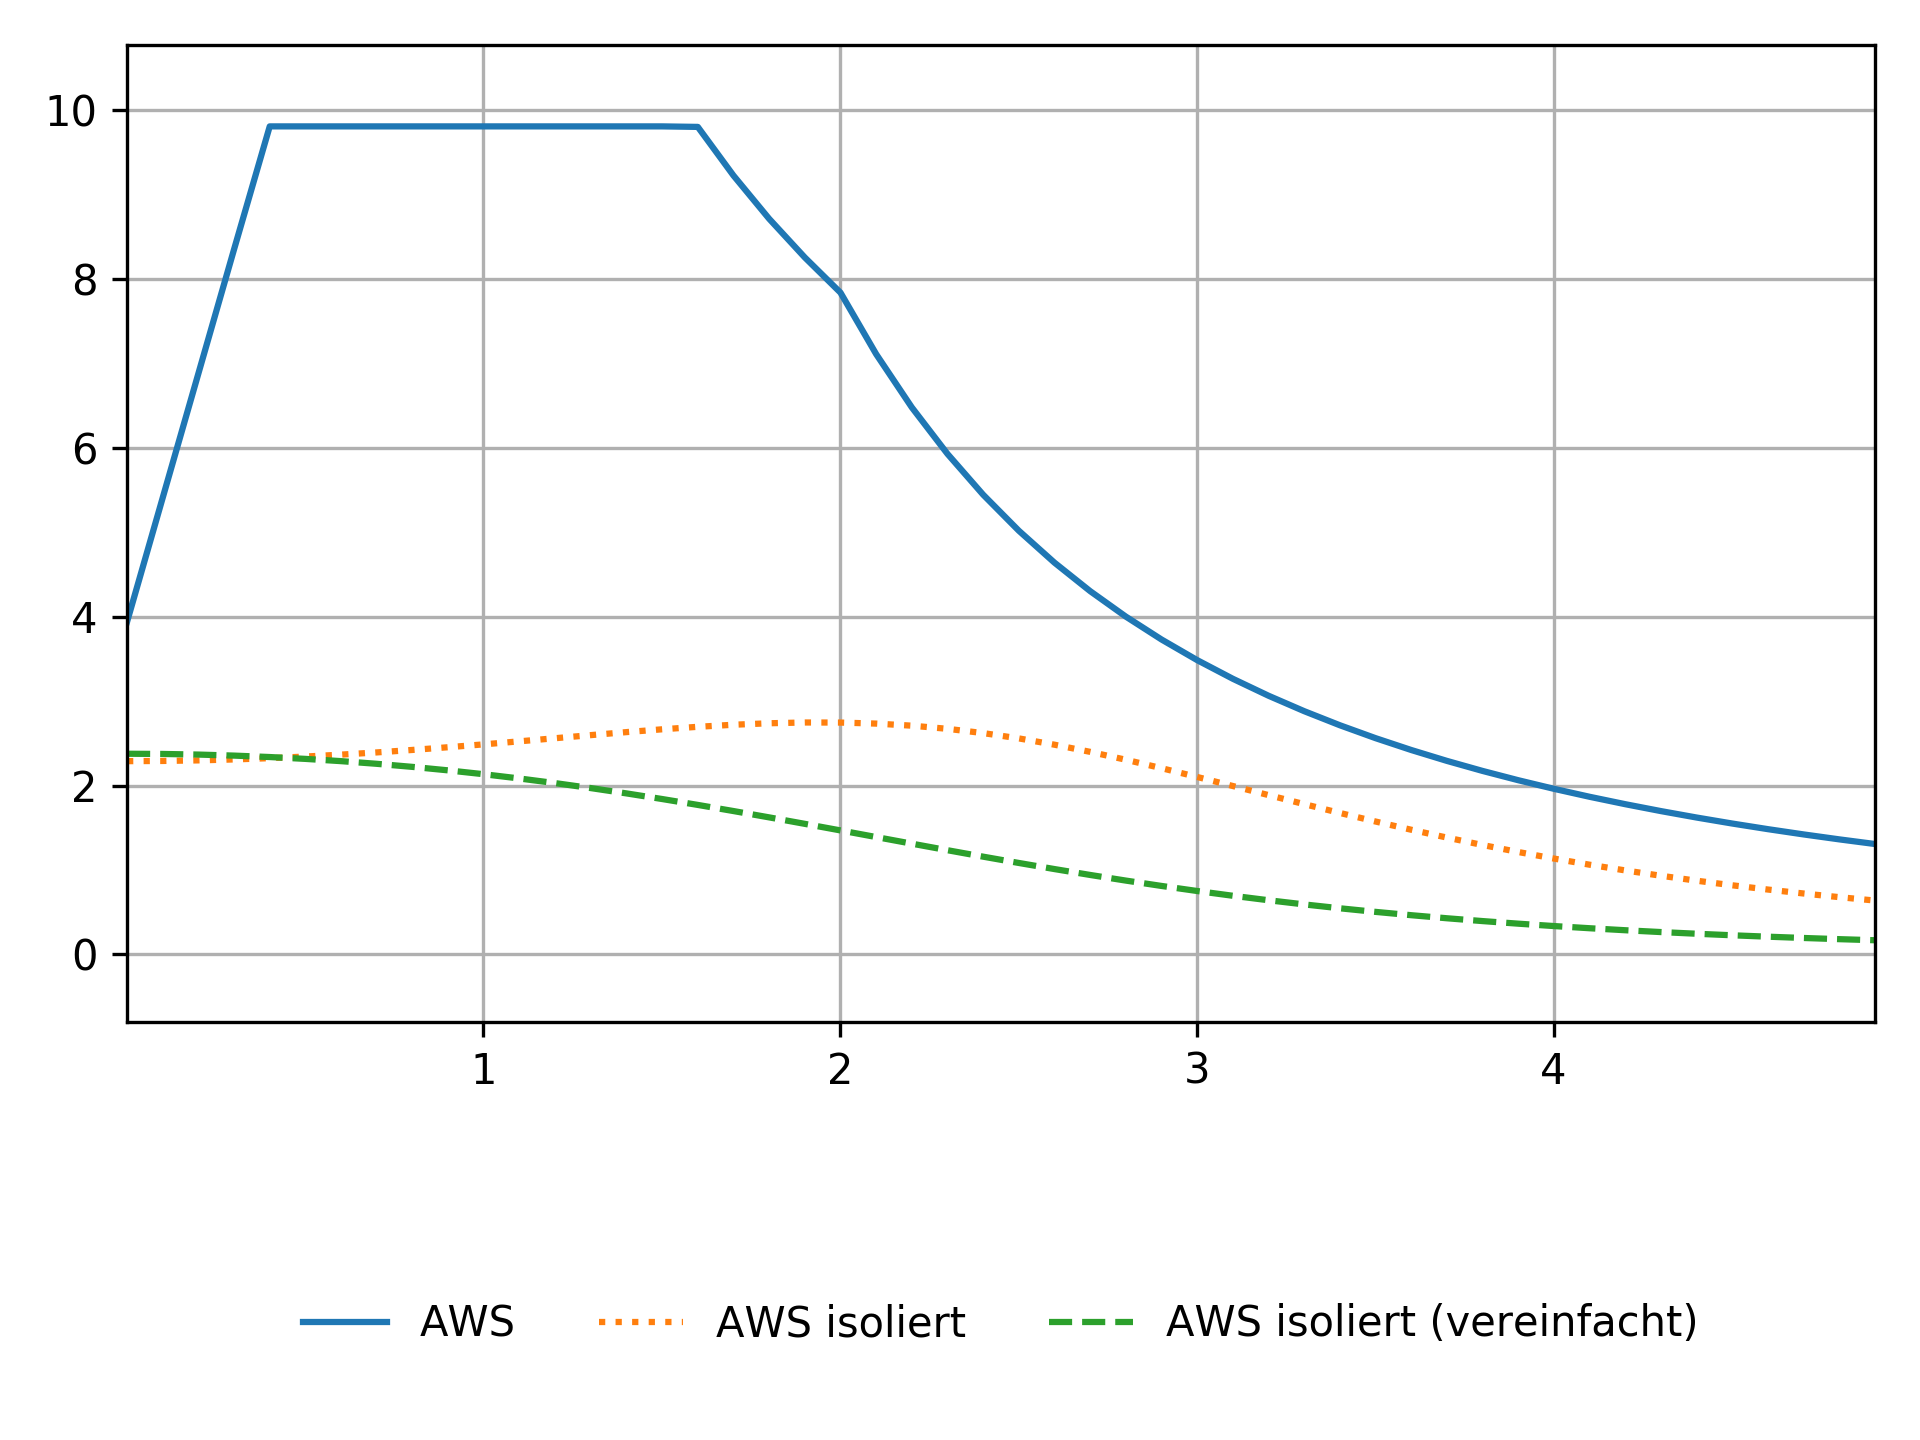
\includegraphics[width=1.0\textwidth]{Isolation.png}
    \caption{Isolationsspektren der drei Ansätze (Beispiel 1)}
    \label{fig:Isolation}
\end{figure}

Wie zu erwarten war, ist die Modellierung als effektiver Einmassenschwinger nur eine Näherung. Die Ergebnisse über die Transmissibilität liefern durchweg größere Beschleunigungen als der vereinfachte Ansatz, wobei sich diese Differenz in der Nähe der Isolatorperiode stärker ausprägt. Auch ist anzumerken, dass die Isolationsspektren geglättet sind, da sie aus dem ebenfalls bereits geglätteten Antwortspektrum berechnet wurden.

\section{Vergleich mit den Ergebnissen einer Zeitschrittberechnung}

Um auch einen Vergleich mit den numerisch ermittelten Werten aus \cite{Isemann} zu machen, wurde das Beispiel in Kapitel 11.3 untersucht.
Mit den angegebenen Massen und der Isolatorsteifigkeit stimmt jedoch die Periode des Isolators, die mit $T = 2.251 s$ angegeben wurde, nicht überein.

\begin{align*}
T &= \frac{2 \pi}{\sqrt{(k_2/(m_2+m_1))}}\\
  &= \frac{2 \pi}{\sqrt{(32000/( 2846.7 t + 1619.5 t)}}\\
  &= 2.347 s \neq 2.251 s
\end{align*}

Die Vermutung liegt nahe, dass für $m_1$ die Masse aus dem vorrangegangenen Beispiel in den Berechnungen verwendet wurde und es sich in den Angaben um einen \glqq Zahlendreher\grqq{} handelt.

\begin{align*}
T &= \frac{2 \pi}{\sqrt{(32000/( 2486.7 t + 1619.5 t)}}\\
  &= 2.251 s = 2.251 s
\end{align*}

Mit dieser bestätigten Vermutung wird weiterhin mit $m_1 = 2486.7 t$ gerechnet.
Aus der angegebenen Steifigkeit für den Isolator von $k_2 = 32000 kN/m$ lässt sich der verwendete Radius und das Dämpfungsmaß bestimmen.

\begin{align*}
k_2 &= \frac{G}{R} + \mu \frac{G}{D}\\
    &= \frac{41062 kN}{R} + 0.05 \cdot \frac{41062 kN}{0.325 m} = 32000 kN/m \Rightarrow R \approx 1.599 m
\end{align*}

\begin{equation*}
\xi_2 = \xi_{eff} = \frac{2}{\pi} \frac{\mu R}{(D + \mu R)} = \frac{2}{\pi} \frac{0.05 \cdot 1.599 m}{(0.325 m + 0.05 \cdot 1.599 m)} \approx 0.1257
\end{equation*} 

\pagebreak

Damit stehen die Parameter fest und die Spektren können erzeugt werden.

\makebox[1cm]{$D$}    = 0.325 m \par
\makebox[1cm]{$\mu$}  = 0.05\par
\makebox[1cm]{$m_1$}  = 2486.7 t\par
\makebox[1cm]{$m_2$}  = 1619.5 t\par
\makebox[1cm]{$k_2$}  = 32000 kN/m \par
\makebox[1cm]{$R$}    = 1.599 m\par

\begin{figure}[H]
    \centering
    \includegraphics[width=1.0\textwidth]{_Isolation_2.png}
    \caption{Vergleich der Isolationsspektren aus Zeitschrittberechnung \cite{Isemann}, vereinfachten Ansatz und Ansatz der Transmissibilität (Beispiel 2)}
    \label{fig:Isolation}
\end{figure}

Hier wird deutlich, dass der vereinfachte Ansatz auf der unsicheren Seite liegt.
Bei dem Ansatz der Transmissibilität liegt die Vermutung nahe, dass die Bestimmung der Beschleunigung am gedämpften Antwortspektrum eine doppelte Berücksichtigung der Dämpfung zufolge hatte, da diese bereits in den Transmissibilitätskoeffizienten erfasst wurde.
Eine Anpassung (\cref{fig:Isolation2}) mit $\eta = \sqrt{10/(5+0)} = 1.4142$ zeigt, dass das Isolationsspektrum nun eine Einhüllende darstellt, allerdings auch deutlich zu große Werte ergibt.

\begin{figure}[H]
    \centering
    \includegraphics[width=1.0\textwidth]{_Isolation_3.png}
    \caption{Vergleich der Isolationsspektren aus Zeitschrittberechnung \cite{Isemann}, vereinfachten Ansatz und Ansatz der Transmissibilität ($\eta = 1.4142$) (Beispiel 2)}
    \label{fig:Isolation2}
\end{figure}

\section{Korrekturansätze}
\label{sec:Korrekturansaetze}

In \cite{Isemann} wurden verschiedene Ansätze untersucht, das Isolationsspektrum nach oben zu korrigieren.
Auch bei dem Ansatz der Transmissibilität könnte man nun versuchen, die Werte nach unten zu korrigieren. Betrachtet man die Transmissionskoeffizienten (\cref{eq:VT2DOF}), so lässt sich erkennen, dass die Dämpfung auch eine Koppelung darstellt. 

Es soll eine grobe Näherung untersucht werden, nach der die Dämpfungsbeiwerte der beiden Systeme getrennt voneinander bestimmt werden.

\begin{align*}
c_1 &= 2 \xi_1 \sqrt{k_1 m_1}\\
c_2 &= 2 \xi_2 \sqrt{k_2 m_2}
\end{align*}

Die Berechnung der Transmissibilität erfolgt dann am nicht transformierten System.

\begin{equation*}
VT(m_2, k_2, c_2, m_1, k_1, c_1)
\end{equation*} 

\begin{table}[H]
\centering
\begin{tabular}{ |c|c|c| } 
 \hline
 Einmassenschwinger & Vereinfacht & Transmissibilität\\
 \hline\hline
 2.958 $m/s^2$ & 2.858 $m/s^2$ & 3.525 $m/s^2$\\
 \hline
\end{tabular}
\caption{Vergleich der Beschleunigungen aus den drei Ansätzen mit Korrektur (Beispiel 1)}
\end{table}

Die Werte aus dem ersten Beispiel liegen nun deutlich näher zusammen.

\begin{figure}[H]
    \centering
    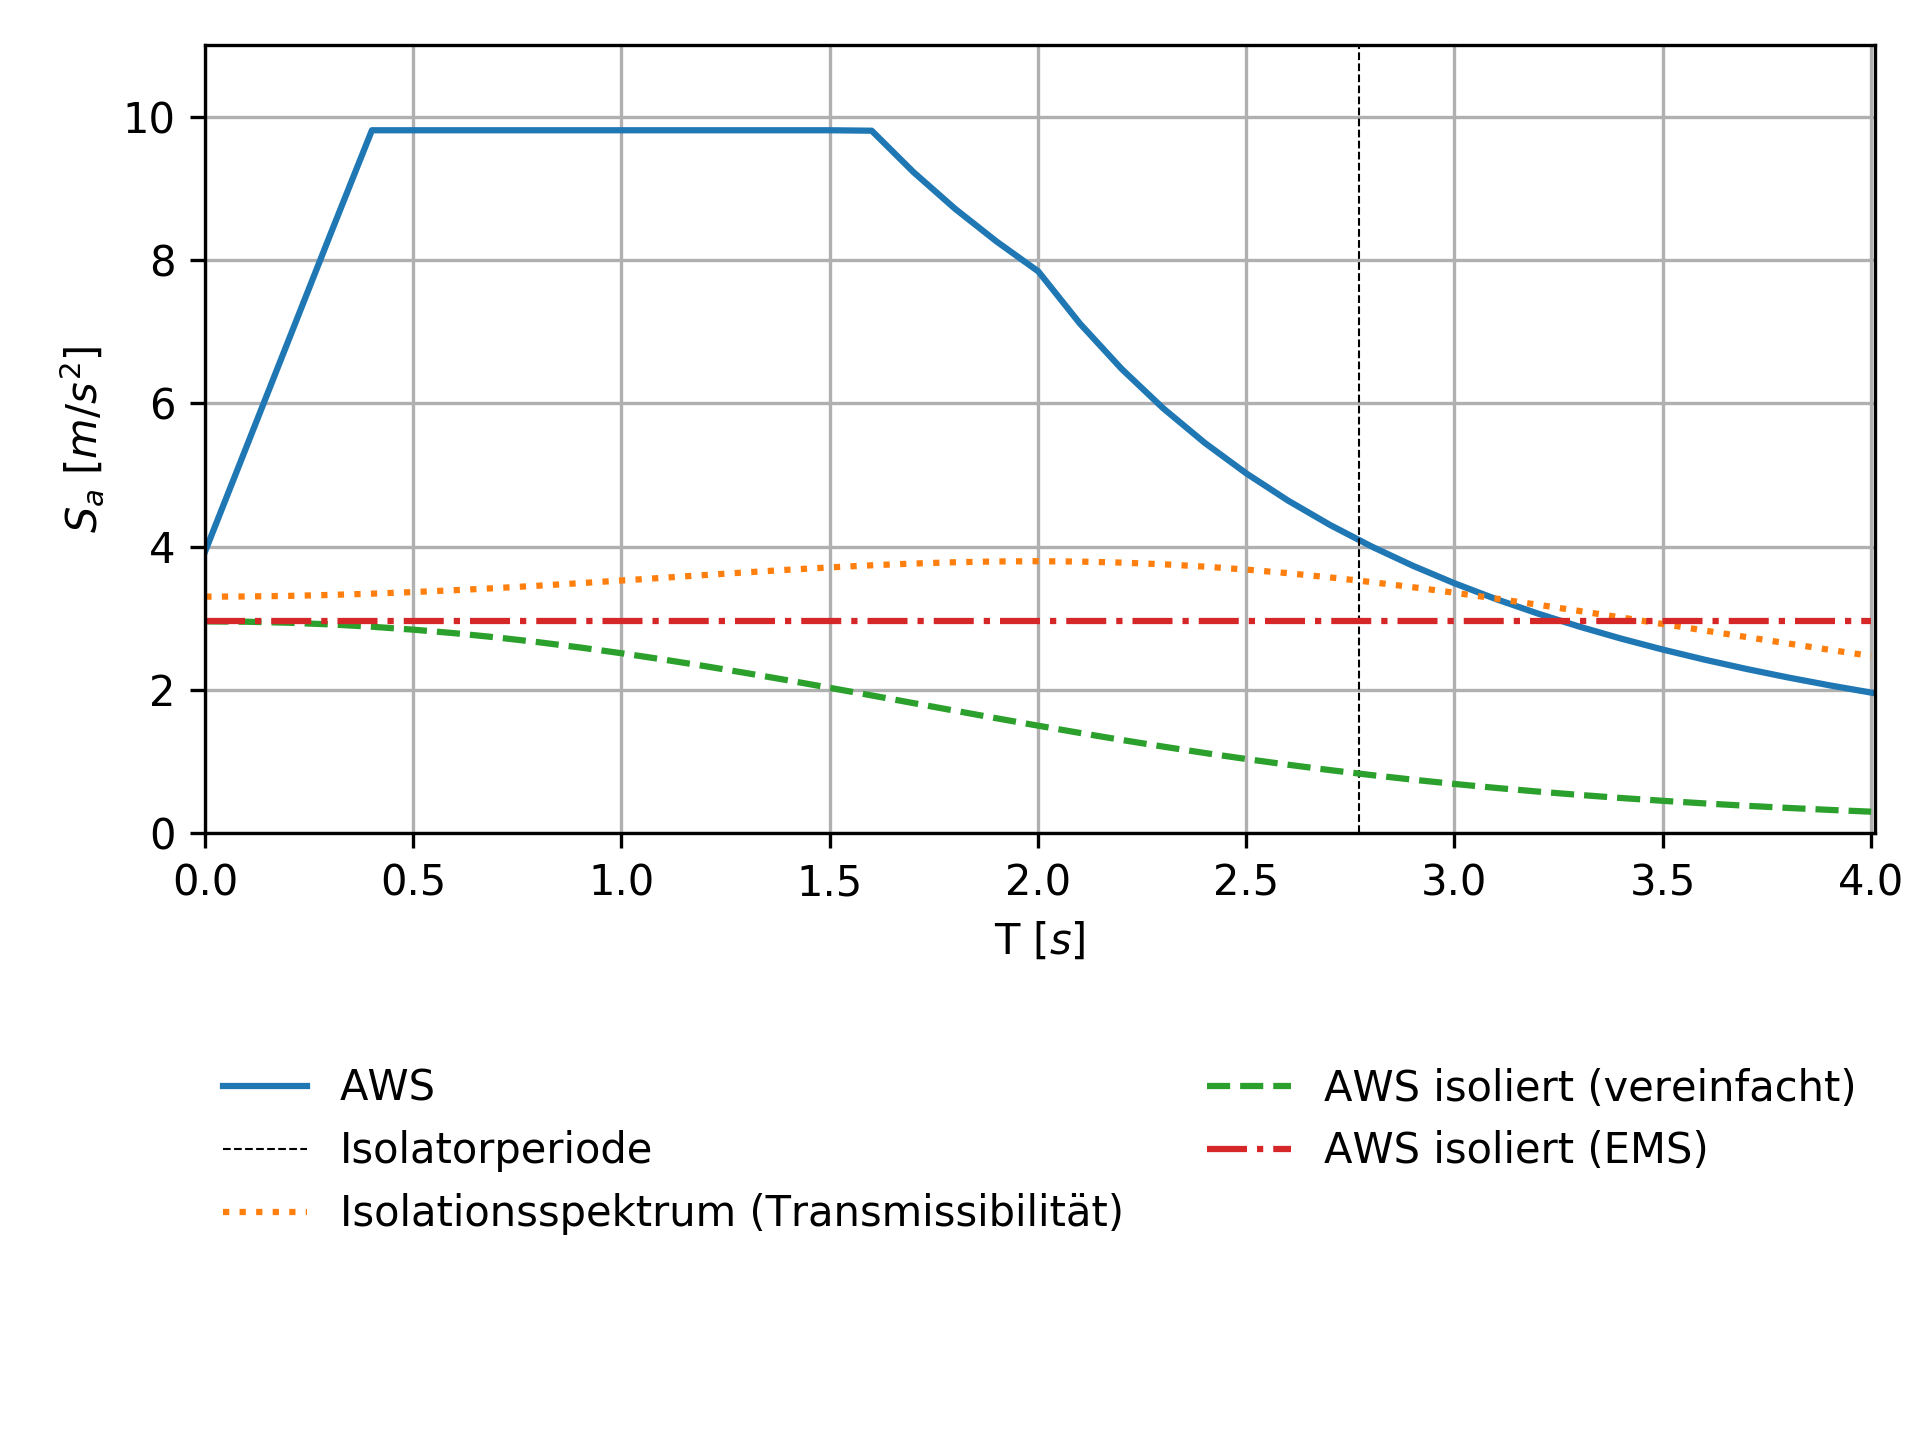
\includegraphics[width=1.0\textwidth]{Isolation_4_2.png}
    \caption{Isolationsspektren der drei Ansätze (Beispiel 1)}
    \label{fig:Isolation2}
\end{figure}


Im zweiten Beispiel (\cref{fig:Isolation21}) kann anhand des Vergleiches der numerischen Werte auch festgestellt werden, dass der qualitative Verlauf besser abgebildet werden konnte.

\begin{figure}[H]
    \centering
    \includegraphics[width=1.0\textwidth]{_Isolation_4.png}
    \caption{Vergleich der Isolationsspektren aus Zeitschrittberechnung \cite{Isemann}, vereinfachten Ansatz und Ansatz der Transmissibilität (Beispiel 2)}
    \label{fig:Isolation21}
\end{figure}

\pagebreak

\chapter{Analyse}
\pagebreak

\chapter{Zusammenfassung}
\pagebreak


\appendix
%\chapter{Appendix}
\cleardoublepage
\phantomsection
\addcontentsline{toc}{chapter}{Nomenklatur}

\chapter*{Nomenklatur}

\begin{longtable}{cp{3cm}p{8cm}}
\hline
Symbol       & Einheit & Beschreibung \\
\hline\hline
$\omega$     & $1/s$   & Kreisfrequenz\\
$T$          & $s$     & Periode      \\
$t$          & $s$     & Zeit         \\
$a$          & $m/s^2$ & Beschleunigung \\
$S_a$        & $m/s^2$ & Spektralbeschleunigung \\
$F$          & $kN$    & Kraft        \\
$u$          & $m$     & Verschiebung \\
$m$          & $t$     & Masse        \\
$M$          & $t$     & Massenmatrix \\
$k$          & $kN/m$  & Steifigkeit  \\
$K$          & $kN/m$  & Steifigkeitsmatrix \\
$E$          & $kN/m^2$& Elastizitätsmodul \\
$I$          & $m^4$   & Flächenmoment 2. Grades \\
$\xi$        & $-$     & Dämpfungsgrad     \\
$c$          & $\frac{kN}{m/s}$     & Dämpfungskoeffizient \\
$C$          & $\frac{kN}{m/s}$     & Dämpfungsmatrix \\
$\eta$       & $-$     & Dämpfungs-Korrekturbeiwert \\
$P$          & $-$     & Wahrscheinlichkeit \\
$\gamma_1$   & $-$     & Bedeutungsbeiwert \\
$G$          & $t, kN$ & Vertikalkraft (Eigengewicht) \\
$D$          & $m$     & Auslenkung \\
$R$          & $m$     & Radius \\
$\theta$     & $^{\circ}$ & Winkel \\
$\mu$        & $-$     & Reibungskoeffizient \\
$\vec{\Phi}$ & $-$     & Eigenvektor \\
$\varphi$    & $-$     & Eigenvektorkomponente \\
$L$          & $-$     & Beteiligunsfaktor \\
$\vec{I}$    & $-$     & Einheitsvektor \\
$VT$         & $-$     & Transmissibilität \\
\hline
\end{longtable}


\cleardoublepage
\phantomsection
\addcontentsline{toc}{chapter}{\listfigurename}
\listoffigures

\cleardoublepage
\phantomsection
\addcontentsline{toc}{chapter}{Bibliographie}
\printbibliography

\cleardoublepage
\phantomsection
\addcontentsline{toc}{chapter}{Eidesstattliche Erklärung}

\chapter*{Eidesstattliche Erklärung}

Hiermit versichere ich, die vorliegende Master-Thesis ohne Hilfe Dritter und nur mit den
angegebenen Quellen und Hilfsmitteln angefertigt zu haben. Alle Stellen, die den
Quellen entnommen wurden, sind als solche kenntlich gemacht worden.

\vspace*{\fill}

\begin{tabular}{@{}p{.5in}p{4in}@{}}
& \hrulefill \\
& \GetAuthor \\
& \date{\today{}, Karlsruhe}\\
\end{tabular}

\vspace*{\fill}

\addtocontents{toc}{\cftpagenumbersoff{chapter}}
\addtocontents{toc}{\cftpagenumbersoff{section}}

\cleardoublepage
\addcontentsline{toc}{chapter}{Datenträger}
\addcontentsline{toc}{section}{\texttt{Masterthesis\_Arne\_Rick.pdf}}
\addcontentsline{toc}{section}{\texttt{Isolationsspektrum.xlsx}}
\addcontentsline{toc}{section}{\texttt{Ausdruckprotokoll\_-\_RStab.pdf}}

\addtocontents{toc}{\cftpagenumberson{section}} 
\addtocontents{toc}{\cftpagenumberson{chapter}} 

\cleardoublepage
\phantomsection
\addcontentsline{toc}{chapter}{Berechnungsprotokoll Modalanalyse mit RStab}
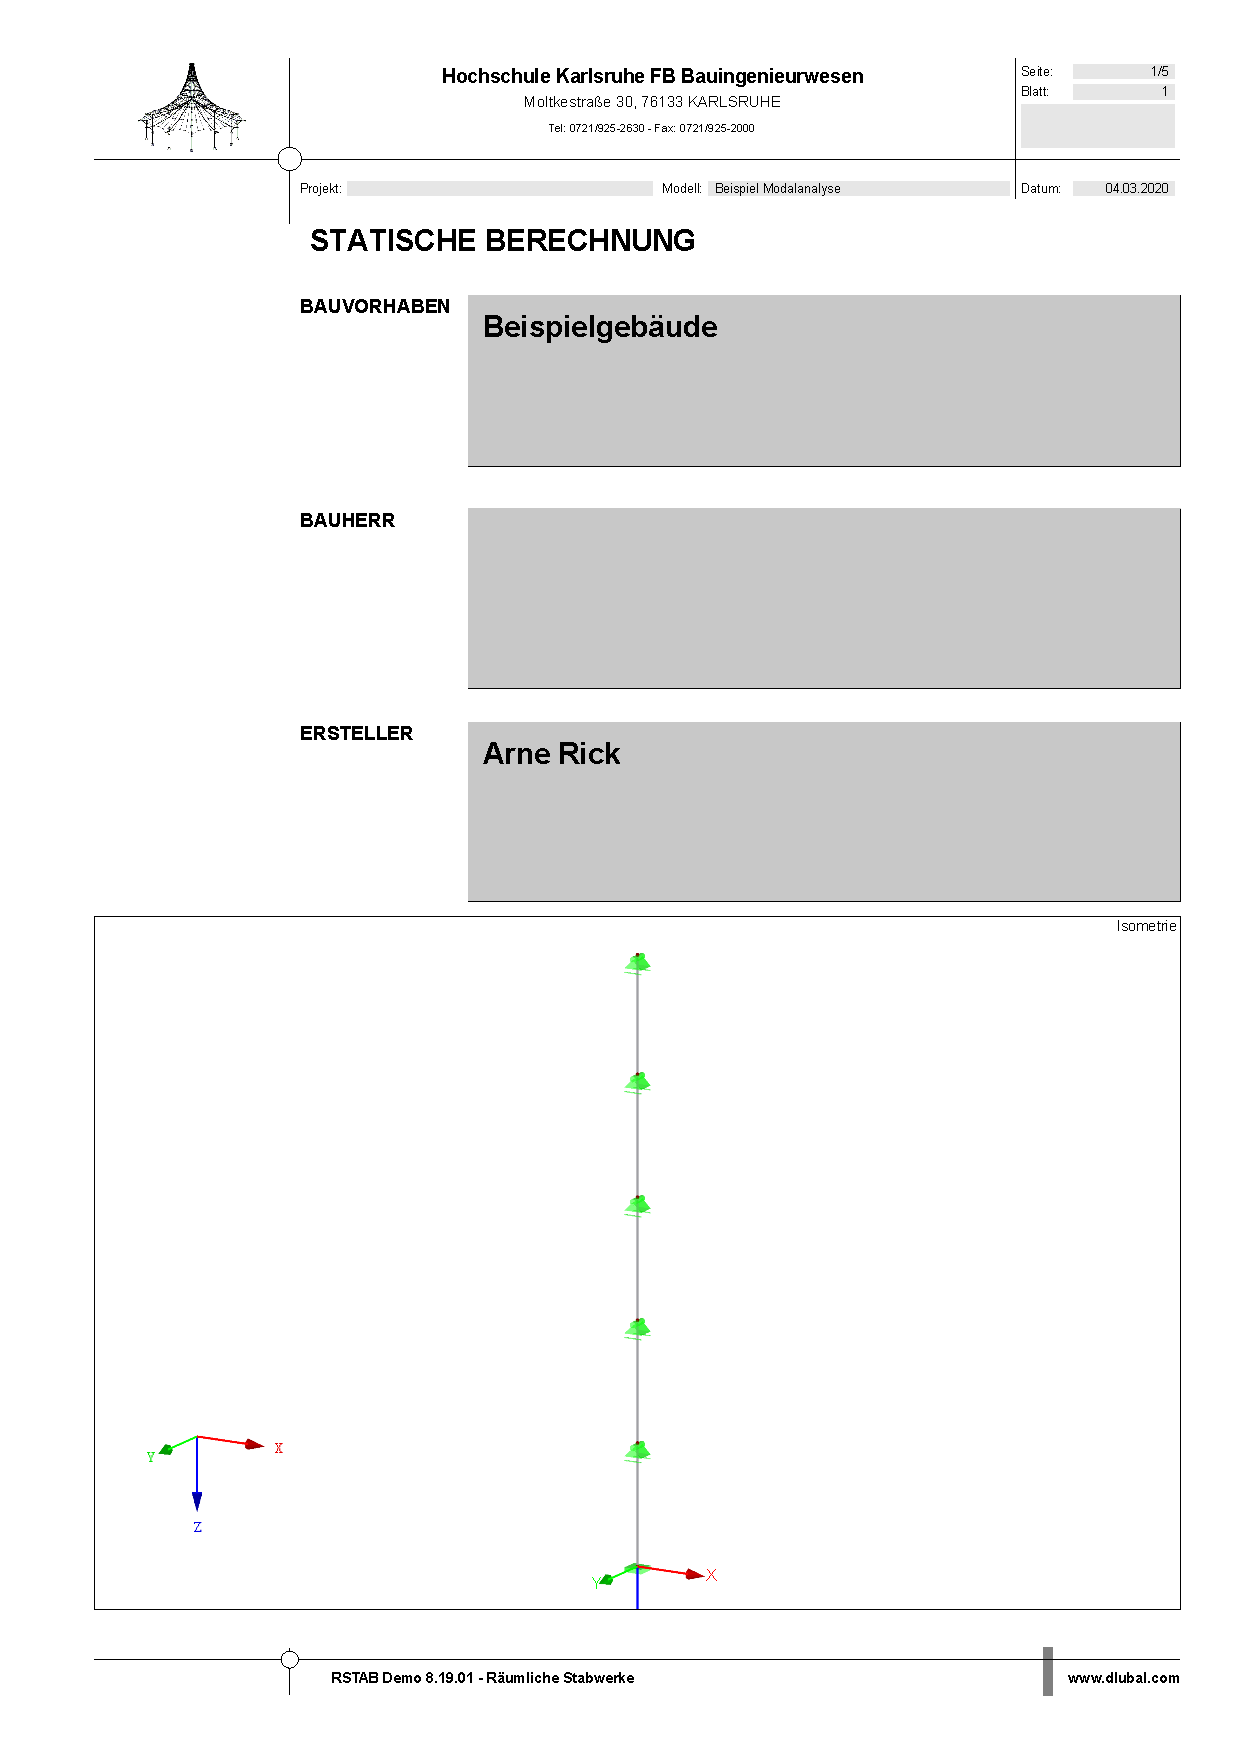
\includepdf[pages=-]{Ausdruckprotokoll_-_RStab.pdf}




\end{document}